\documentclass{beamer}
%%\documentclass[20pt]{beamer}

%%\geometry{papersize={720pt, 540pt}}

\usepackage{tikz}
\usepackage{pgf-umlsd}
\usepackage[normalem]{ulem}
\usepackage{array}
\usepackage{listings}
\usepackage{adjustbox}

\usetikzlibrary{calc,trees,positioning,arrows,chains,%
  decorations.pathreplacing,decorations.pathmorphing,decorations.markings,%
  matrix,graphs,shapes.geometric,shapes.multipart,patterns,fit,
  shapes.callouts}

% Fixed-width columns for tabular.
\newcolumntype{L}[1]{>{\raggedright\let\newline\\\arraybackslash\hspace{0pt}}m{#1}}
\newcolumntype{C}[1]{>{\centering\let\newline\\\arraybackslash\hspace{0pt}}m{#1}}
\newcolumntype{R}[1]{>{\raggedleft\let\newline\\\arraybackslash\hspace{0pt}}m{#1}}

\usetheme{default}
%%\usecolortheme{crane}

\setbeamertemplate{footline}[text line]{\parbox{\linewidth}{\vspace*{-8pt}\centering\insertpagenumber}}
\setbeamertemplate{navigation symbols}{}

\newcommand{\rcgo}{rc\textsubscript{go}}

% Define Language
\lstdefinelanguage{rcgo}
{
  % list of keywords
  morekeywords={
    type,
    component,
    push,
    pull,
    init,
    action,
    reaction,
    getter,
    $const,
    $foreign,
    bind,
    instance,
    activate,
    heap,
    change,
    var,
    new,
    move,
    merge
  },
  morecomment=[l]{//},
  morecomment=[s]{/*}{*/}
}

\definecolor{eclipseGreen}{RGB}{63,127,95}
\definecolor{eclipseBlue}{RGB}{42,0.0,255}
\definecolor{eclipsePurple}{RGB}{127,0,85}

\lstset{
  language={rcgo},
  basicstyle=\small\ttfamily,
  columns=fixed,
  keywordstyle=\color{eclipseBlue},
  commentstyle=\color{eclipseGreen},
}

% Shapes for diagrams.
\makeatletter
\pgfdeclareshape{rightout}{
  \savedanchor{\center}{
    \pgfpointorigin
  }
  \savedanchor{\text}{
    \pgfpointorigin
    \pgf@x=-\wd\pgfnodeparttextbox
    \pgfutil@tempdima=-\dp\pgfnodeparttextbox
    \advance\pgf@y by\pgfutil@tempdima/
  }
  \savedanchor{\southwest}{
    \pgf@x=-\wd\pgfnodeparttextbox
    \pgf@y=-.5\ht\pgfnodeparttextbox
    \pgfutil@tempdima=-.5\dp\pgfnodeparttextbox
    \advance\pgf@y by\pgfutil@tempdima
    \pgfmathsetlength{\pgf@xb}{\pgfkeysvalueof{/pgf/inner xsep}}%
    \pgfmathsetlength{\pgf@yb}{\pgfkeysvalueof{/pgf/inner ysep}}%
    \advance\pgf@x by-\pgf@xb
    \advance\pgf@y by-\pgf@yb
  }
  \savedanchor{\south}{
    \pgf@x=-.5\wd\pgfnodeparttextbox
    \pgf@y=-.5\ht\pgfnodeparttextbox
    \pgfutil@tempdima=-.5\dp\pgfnodeparttextbox
    \advance\pgf@y by\pgfutil@tempdima
    \pgfmathsetlength{\pgf@yb}{\pgfkeysvalueof{/pgf/inner ysep}}%
    \advance\pgf@y by-\pgf@yb
  }
  \savedanchor{\northwest}{
    \pgf@x=-\wd\pgfnodeparttextbox
    \pgfutil@tempdima=.5\dp\pgfnodeparttextbox
    \pgf@y=.5\ht\pgfnodeparttextbox \advance\pgf@y by\pgfutil@tempdima
    \pgfmathsetlength{\pgf@xb}{\pgfkeysvalueof{/pgf/inner xsep}}%
    \pgfmathsetlength{\pgf@yb}{\pgfkeysvalueof{/pgf/inner ysep}}%
    \advance\pgf@x by-\pgf@xb
    \advance\pgf@y by\pgf@yb
  }
  \savedanchor{\north}{
    \pgf@x=-.5\wd\pgfnodeparttextbox
    \pgfutil@tempdima=.5\dp\pgfnodeparttextbox
    \pgf@y=.5\ht\pgfnodeparttextbox \advance\pgf@y by\pgfutil@tempdima
    \pgfmathsetlength{\pgf@yb}{\pgfkeysvalueof{/pgf/inner ysep}}%
    \advance\pgf@y by\pgf@yb
  }
  \savedanchor{\west}{
    \pgfpointorigin
    \pgf@x=-\wd\pgfnodeparttextbox
    \pgfmathsetlength{\pgf@xb}{\pgfkeysvalueof{/pgf/inner xsep}}%
    \advance\pgf@x by-\pgf@xb
  }
  \savedanchor{\southeast}{
    \pgfpointorigin
    \pgfutil@tempdima=-.5\dp\pgfnodeparttextbox
    \pgf@y=-.5\ht\pgfnodeparttextbox \advance\pgf@y by\pgfutil@tempdima
    \pgfmathsetlength{\pgf@xb}{\pgfkeysvalueof{/pgf/inner xsep}}%
    \pgfmathsetlength{\pgf@yb}{\pgfkeysvalueof{/pgf/inner ysep}}%
    \advance\pgf@x by\pgf@xb
    \advance\pgf@y by-\pgf@yb
  }
  \savedanchor{\northeast}{
    \pgfpointorigin
    \pgfutil@tempdima=.5\dp\pgfnodeparttextbox
    \pgf@y=.5\ht\pgfnodeparttextbox \advance\pgf@y by\pgfutil@tempdima
    \pgfmathsetlength{\pgf@xb}{\pgfkeysvalueof{/pgf/inner xsep}}%
    \pgfmathsetlength{\pgf@yb}{\pgfkeysvalueof{/pgf/inner ysep}}%
    \advance\pgf@x by\pgf@xb
    \advance\pgf@y by\pgf@yb
  }
  \savedanchor{\east}{
    \pgfpointorigin
    \pgfutil@tempdima=.5\ht\pgfnodeparttextbox
    \advance\pgf@x by\pgfutil@tempdima
    \pgfutil@tempdima=.5\dp\pgfnodeparttextbox
    \advance\pgf@x by\pgfutil@tempdima
    \pgfmathsetlength{\pgf@xb}{\pgfkeysvalueof{/pgf/inner xsep}}%
    \advance\pgf@x by\pgf@xb
  }

  \anchor{center}{\center}
  \anchor{text}{\text}

  \anchor{south west}{\southwest}
  \anchor{west}{\west}
  \anchor{north west}{\northwest}
  \anchor{north}{\north}
  \anchor{north east}{\northeast}
  \anchor{east}{\east}
  \anchor{south east}{\southeast}
  \anchor{south}{\south}

  \backgroundpath{
    \pgfmoveto{\southwest}
    \pgflineto{\west}
    \pgflineto{\northwest}
    \pgflineto{\north}
    \pgflineto{\northeast}
    \pgflineto{\east}
    \pgflineto{\southeast}
    \pgflineto{\south}
    \pgflineto{\southwest}
  }
}
\makeatother

\makeatletter
\pgfdeclareshape{rightin}{
  \savedanchor{\center}{
    \pgfpointorigin
  }
  \savedanchor{\text}{
    \pgfpointorigin
    \pgf@x=-\wd\pgfnodeparttextbox
    \pgfutil@tempdima=-\dp\pgfnodeparttextbox
    \advance\pgf@y by\pgfutil@tempdima/
  }
  \savedanchor{\southwest}{
    \pgf@x=-\wd\pgfnodeparttextbox
    \pgf@y=-.5\ht\pgfnodeparttextbox
    \pgfutil@tempdima=-.5\dp\pgfnodeparttextbox
    \advance\pgf@y by\pgfutil@tempdima
    \pgfmathsetlength{\pgf@xb}{\pgfkeysvalueof{/pgf/inner xsep}}%
    \pgfmathsetlength{\pgf@yb}{\pgfkeysvalueof{/pgf/inner ysep}}%
    \advance\pgf@x by-\pgf@xb
    \advance\pgf@y by-\pgf@yb
  }
  \savedanchor{\south}{
    \pgf@x=-.5\wd\pgfnodeparttextbox
    \pgf@y=-.5\ht\pgfnodeparttextbox
    \pgfutil@tempdima=-.5\dp\pgfnodeparttextbox
    \advance\pgf@y by\pgfutil@tempdima
    \pgfmathsetlength{\pgf@yb}{\pgfkeysvalueof{/pgf/inner ysep}}%
    \advance\pgf@y by-\pgf@yb
  }
  \savedanchor{\northwest}{
    \pgf@x=-\wd\pgfnodeparttextbox
    \pgfutil@tempdima=.5\dp\pgfnodeparttextbox
    \pgf@y=.5\ht\pgfnodeparttextbox \advance\pgf@y by\pgfutil@tempdima
    \pgfmathsetlength{\pgf@xb}{\pgfkeysvalueof{/pgf/inner xsep}}%
    \pgfmathsetlength{\pgf@yb}{\pgfkeysvalueof{/pgf/inner ysep}}%
    \advance\pgf@x by-\pgf@xb
    \advance\pgf@y by\pgf@yb
  }
  \savedanchor{\north}{
    \pgf@x=-.5\wd\pgfnodeparttextbox
    \pgfutil@tempdima=.5\dp\pgfnodeparttextbox
    \pgf@y=.5\ht\pgfnodeparttextbox \advance\pgf@y by\pgfutil@tempdima
    \pgfmathsetlength{\pgf@yb}{\pgfkeysvalueof{/pgf/inner ysep}}%
    \advance\pgf@y by\pgf@yb
  }
  \savedanchor{\west}{
    \pgfpointorigin
    \pgf@x=-\wd\pgfnodeparttextbox
    \pgfmathsetlength{\pgf@xb}{\pgfkeysvalueof{/pgf/inner xsep}}%
    \advance\pgf@x by-\pgf@xb
  }
  \savedanchor{\southeast}{
    \pgfpointorigin
    \pgfutil@tempdima=-.5\dp\pgfnodeparttextbox
    \pgf@y=-.5\ht\pgfnodeparttextbox \advance\pgf@y by\pgfutil@tempdima
    \pgfmathsetlength{\pgf@xb}{\pgfkeysvalueof{/pgf/inner xsep}}%
    \pgfmathsetlength{\pgf@yb}{\pgfkeysvalueof{/pgf/inner ysep}}%
    \advance\pgf@x by\pgf@xb
    \advance\pgf@y by-\pgf@yb
    \pgfutil@tempdima=.5\ht\pgfnodeparttextbox
    \advance\pgf@x by\pgfutil@tempdima
    \pgfutil@tempdima=.5\dp\pgfnodeparttextbox
    \advance\pgf@x by\pgfutil@tempdima
  }
  \savedanchor{\northeast}{
    \pgfpointorigin
    \pgfutil@tempdima=.5\dp\pgfnodeparttextbox
    \pgf@y=.5\ht\pgfnodeparttextbox \advance\pgf@y by\pgfutil@tempdima
    \pgfmathsetlength{\pgf@xb}{\pgfkeysvalueof{/pgf/inner xsep}}%
    \pgfmathsetlength{\pgf@yb}{\pgfkeysvalueof{/pgf/inner ysep}}%
    \advance\pgf@x by\pgf@xb
    \advance\pgf@y by\pgf@yb
    \pgfutil@tempdima=.5\ht\pgfnodeparttextbox
    \advance\pgf@x by\pgfutil@tempdima
    \pgfutil@tempdima=.5\dp\pgfnodeparttextbox
    \advance\pgf@x by\pgfutil@tempdima
  }
  \savedanchor{\east}{
    \pgfpointorigin
    \pgfmathsetlength{\pgf@xb}{\pgfkeysvalueof{/pgf/inner xsep}}%
    \advance\pgf@x by\pgf@xb
  }

  \anchor{center}{\center}
  \anchor{text}{\text}

  \anchor{south west}{\southwest}
  \anchor{west}{\west}
  \anchor{north west}{\northwest}
  \anchor{north}{\north}
  \anchor{north east}{\northeast}
  \anchor{east}{\east}
  \anchor{south east}{\southeast}
  \anchor{south}{\south}

  \backgroundpath{
    \pgfmoveto{\southwest}
    \pgflineto{\west}
    \pgflineto{\northwest}
    \pgflineto{\north}
    \pgflineto{\northeast}
    \pgflineto{\east}
    \pgflineto{\southeast}
    \pgflineto{\south}
    \pgflineto{\southwest}
  }
}
\makeatother

\makeatletter
\pgfdeclareshape{leftout}{
  \savedanchor{\center}{
    \pgfpointorigin
  }
  \savedanchor{\text}{
    \pgfpointorigin
    \pgfutil@tempdima=-\dp\pgfnodeparttextbox
    \advance\pgf@y by\pgfutil@tempdima/
  }
  \savedanchor{\southeast}{
    \pgf@x=\wd\pgfnodeparttextbox
    \pgf@y=-.5\ht\pgfnodeparttextbox
    \pgfutil@tempdima=-.5\dp\pgfnodeparttextbox
    \advance\pgf@y by\pgfutil@tempdima
    \pgfmathsetlength{\pgf@xb}{\pgfkeysvalueof{/pgf/inner xsep}}%
    \pgfmathsetlength{\pgf@yb}{\pgfkeysvalueof{/pgf/inner ysep}}%
    \advance\pgf@x by\pgf@xb
    \advance\pgf@y by-\pgf@yb
  }
  \savedanchor{\south}{
    \pgf@x=.5\wd\pgfnodeparttextbox
    \pgf@y=-.5\ht\pgfnodeparttextbox
    \pgfutil@tempdima=-.5\dp\pgfnodeparttextbox
    \advance\pgf@y by\pgfutil@tempdima
    \pgfmathsetlength{\pgf@yb}{\pgfkeysvalueof{/pgf/inner ysep}}%
    \advance\pgf@y by-\pgf@yb
  }
  \savedanchor{\northeast}{
    \pgf@x=\wd\pgfnodeparttextbox
    \pgfutil@tempdima=.5\dp\pgfnodeparttextbox
    \pgf@y=.5\ht\pgfnodeparttextbox \advance\pgf@y by\pgfutil@tempdima
    \pgfmathsetlength{\pgf@xb}{\pgfkeysvalueof{/pgf/inner xsep}}%
    \pgfmathsetlength{\pgf@yb}{\pgfkeysvalueof{/pgf/inner ysep}}%
    \advance\pgf@x by\pgf@xb
    \advance\pgf@y by\pgf@yb
  }
  \savedanchor{\north}{
    \pgf@x=.5\wd\pgfnodeparttextbox
    \pgfutil@tempdima=.5\dp\pgfnodeparttextbox
    \pgf@y=.5\ht\pgfnodeparttextbox \advance\pgf@y by\pgfutil@tempdima
    \pgfmathsetlength{\pgf@yb}{\pgfkeysvalueof{/pgf/inner ysep}}%
    \advance\pgf@y by\pgf@yb
  }
  \savedanchor{\east}{
    \pgfpointorigin
    \pgf@x=\wd\pgfnodeparttextbox
    \pgfmathsetlength{\pgf@xb}{\pgfkeysvalueof{/pgf/inner xsep}}%
    \advance\pgf@x by\pgf@xb
  }
  \savedanchor{\southwest}{
    \pgfpointorigin
    \pgfutil@tempdima=-.5\dp\pgfnodeparttextbox
    \pgf@y=-.5\ht\pgfnodeparttextbox \advance\pgf@y by\pgfutil@tempdima
    \pgfmathsetlength{\pgf@xb}{\pgfkeysvalueof{/pgf/inner xsep}}%
    \pgfmathsetlength{\pgf@yb}{\pgfkeysvalueof{/pgf/inner ysep}}%
    \advance\pgf@x by-\pgf@xb
    \advance\pgf@y by-\pgf@yb
  }
  \savedanchor{\northwest}{
    \pgfpointorigin
    \pgfutil@tempdima=.5\dp\pgfnodeparttextbox
    \pgf@y=.5\ht\pgfnodeparttextbox \advance\pgf@y by\pgfutil@tempdima
    \pgfmathsetlength{\pgf@xb}{\pgfkeysvalueof{/pgf/inner xsep}}%
    \pgfmathsetlength{\pgf@yb}{\pgfkeysvalueof{/pgf/inner ysep}}%
    \advance\pgf@x by-\pgf@xb
    \advance\pgf@y by\pgf@yb
  }
  \savedanchor{\west}{
    \pgfpointorigin
    \pgfutil@tempdima=.5\ht\pgfnodeparttextbox
    \advance\pgf@x by-\pgfutil@tempdima
    \pgfutil@tempdima=.5\dp\pgfnodeparttextbox
    \advance\pgf@x by-\pgfutil@tempdima
    \pgfmathsetlength{\pgf@xb}{\pgfkeysvalueof{/pgf/inner xsep}}%
    \advance\pgf@x by-\pgf@xb
  }

  \anchor{center}{\center}
  \anchor{text}{\text}

  \anchor{south west}{\southwest}
  \anchor{west}{\west}
  \anchor{north west}{\northwest}
  \anchor{north}{\north}
  \anchor{north east}{\northeast}
  \anchor{east}{\east}
  \anchor{south east}{\southeast}
  \anchor{south}{\south}

  \backgroundpath{
    \pgfmoveto{\southwest}
    \pgflineto{\west}
    \pgflineto{\northwest}
    \pgflineto{\north}
    \pgflineto{\northeast}
    \pgflineto{\east}
    \pgflineto{\southeast}
    \pgflineto{\south}
    \pgflineto{\southwest}
  }
}
\makeatother

\makeatletter
\pgfdeclareshape{leftin}{
  \savedanchor{\center}{
    \pgfpointorigin
  }
  \savedanchor{\text}{
    \pgfpointorigin
    \pgfutil@tempdima=-\dp\pgfnodeparttextbox
    \advance\pgf@y by\pgfutil@tempdima/
  }
  \savedanchor{\southwest}{
    \pgfpointorigin
    \pgfutil@tempdima=-.5\dp\pgfnodeparttextbox
    \pgf@y=-.5\ht\pgfnodeparttextbox \advance\pgf@y by\pgfutil@tempdima
    \pgfmathsetlength{\pgf@xb}{\pgfkeysvalueof{/pgf/inner xsep}}%
    \pgfmathsetlength{\pgf@yb}{\pgfkeysvalueof{/pgf/inner ysep}}%
    \advance\pgf@x by-\pgf@xb
    \advance\pgf@y by-\pgf@yb
    \pgfutil@tempdima=.5\ht\pgfnodeparttextbox
    \advance\pgf@x by-\pgfutil@tempdima
    \pgfutil@tempdima=.5\dp\pgfnodeparttextbox
    \advance\pgf@x by-\pgfutil@tempdima
  }
  \savedanchor{\northwest}{
    \pgfpointorigin
    \pgfutil@tempdima=.5\dp\pgfnodeparttextbox
    \pgf@y=.5\ht\pgfnodeparttextbox \advance\pgf@y by\pgfutil@tempdima
    \pgfmathsetlength{\pgf@xb}{\pgfkeysvalueof{/pgf/inner xsep}}%
    \pgfmathsetlength{\pgf@yb}{\pgfkeysvalueof{/pgf/inner ysep}}%
    \advance\pgf@x by-\pgf@xb
    \advance\pgf@y by\pgf@yb
    \pgfutil@tempdima=.5\ht\pgfnodeparttextbox
    \advance\pgf@x by-\pgfutil@tempdima
    \pgfutil@tempdima=.5\dp\pgfnodeparttextbox
    \advance\pgf@x by-\pgfutil@tempdima
  }
  \savedanchor{\west}{
    \pgfpointorigin
    \pgfmathsetlength{\pgf@xb}{\pgfkeysvalueof{/pgf/inner xsep}}%
    \advance\pgf@x by-\pgf@xb
  }
  \savedanchor{\southeast}{
    \pgf@x=\wd\pgfnodeparttextbox
    \pgf@y=-.5\ht\pgfnodeparttextbox
    \pgfutil@tempdima=-.5\dp\pgfnodeparttextbox
    \advance\pgf@y by\pgfutil@tempdima
    \pgfmathsetlength{\pgf@xb}{\pgfkeysvalueof{/pgf/inner xsep}}%
    \pgfmathsetlength{\pgf@yb}{\pgfkeysvalueof{/pgf/inner ysep}}%
    \advance\pgf@x by\pgf@xb
    \advance\pgf@y by-\pgf@yb
  }
  \savedanchor{\south}{
    \pgf@x=.5\wd\pgfnodeparttextbox
    \pgf@y=-.5\ht\pgfnodeparttextbox
    \pgfutil@tempdima=-.5\dp\pgfnodeparttextbox
    \advance\pgf@y by\pgfutil@tempdima
    \pgfmathsetlength{\pgf@yb}{\pgfkeysvalueof{/pgf/inner ysep}}%
    \advance\pgf@y by-\pgf@yb
  }
  \savedanchor{\northeast}{
    \pgf@x=\wd\pgfnodeparttextbox
    \pgfutil@tempdima=.5\dp\pgfnodeparttextbox
    \pgf@y=.5\ht\pgfnodeparttextbox \advance\pgf@y by\pgfutil@tempdima
    \pgfmathsetlength{\pgf@xb}{\pgfkeysvalueof{/pgf/inner xsep}}%
    \pgfmathsetlength{\pgf@yb}{\pgfkeysvalueof{/pgf/inner ysep}}%
    \advance\pgf@x by\pgf@xb
    \advance\pgf@y by\pgf@yb
  }
  \savedanchor{\north}{
    \pgf@x=.5\wd\pgfnodeparttextbox
    \pgfutil@tempdima=.5\dp\pgfnodeparttextbox
    \pgf@y=.5\ht\pgfnodeparttextbox \advance\pgf@y by\pgfutil@tempdima
    \pgfmathsetlength{\pgf@yb}{\pgfkeysvalueof{/pgf/inner ysep}}%
    \advance\pgf@y by\pgf@yb
  }
  \savedanchor{\east}{
    \pgfpointorigin
    \pgf@x=\wd\pgfnodeparttextbox
    \pgfmathsetlength{\pgf@xb}{\pgfkeysvalueof{/pgf/inner xsep}}%
    \advance\pgf@x by\pgf@xb
  }

  \anchor{center}{\center}
  \anchor{text}{\text}

  \anchor{south west}{\southwest}
  \anchor{west}{\west}
  \anchor{north west}{\northwest}
  \anchor{north}{\north}
  \anchor{north east}{\northeast}
  \anchor{east}{\east}
  \anchor{south east}{\southeast}
  \anchor{south}{\south}

  \backgroundpath{
    \pgfmoveto{\southwest}
    \pgflineto{\west}
    \pgflineto{\northwest}
    \pgflineto{\north}
    \pgflineto{\northeast}
    \pgflineto{\east}
    \pgflineto{\southeast}
    \pgflineto{\south}
    \pgflineto{\southwest}
  }
}
\makeatother

\title{A Transactional Model and Platform for Designing and Implementing Reactive Systems}
\author{Justin R. Wilson}
%%\institute{\texttt{wilsonj@ociweb.com} \\ Object Computing, Inc.}
\date{}

\begin{document}

\frame{\titlepage

  \begin{center}
    \small
   A dissertation presented to the Graduate School of Arts and Sciences\\
   of Washington University in partial fulfillment of the\\
   requirements for the degree of\\
   Doctor of Philosophy\\
   September 2016\\
   Saint Louis, Missouri
 \end{center}
}

\begin{frame}{Introduction}

  \begin{center}
    {\Large Transformational Programs}
    \vspace*{12pt}

    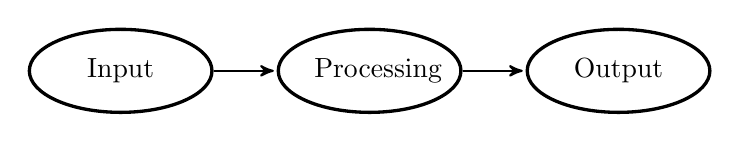
\begin{tikzpicture}
      [>=stealth',
        element/.style={
          ellipse,
          draw=black, very thick,
          text width=4em,
          minimum height=3em,
          text centered,
          on chain},
        line/.style={draw, thick, <-},
        every join/.style={->, thick,shorten >=1pt},
        node distance=.8cm,
        start chain=going right,]
      \node[element, join] (input) {Input};
      \node[element, join] (processing) {Processing};
      \node[element, join] (output) {Output};
    \end{tikzpicture}
  \end{center}

  \rule{\textwidth}{0.4pt}

  \begin{center}
    {\Large Reactive Programs}
    \vspace*{12pt}

    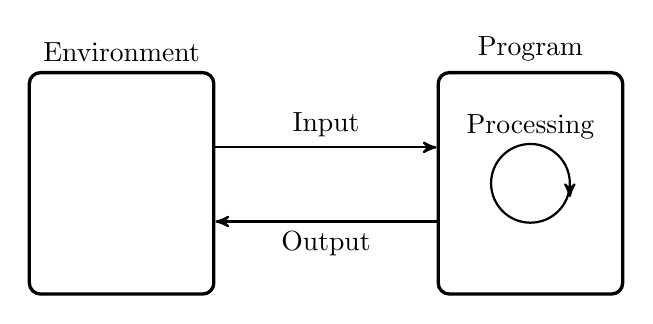
\begin{tikzpicture}
      [>=stealth',
        line/.style={draw, thick, ->},
        entity/.style={
          rectangle,
          rounded corners,
          draw=black, very thick,
          text centered,
          text width=6em,
          minimum height=8em,
}]
      \node[entity, label={Environment}] (environment) {};
      \node[entity, right=4cm, label={Program}] (program) at (environment) {};
      \draw[line] ($(environment.south east)!0.66!(environment.north east)$) -- ($(program.south west)!0.66!(program.north west)$) node [midway, above] {Input};
      \draw[line] ($(program.south west)!0.33!(program.north west)$) -- ($(environment.south east)!0.33!(environment.north east)$) node [midway, below] {Output};

      \draw[line,
        decoration={markings, mark=at position 0.0 with {\arrow{<}}},
        postaction={decorate}
      ]
      (program) circle (0.5) node [label={[label distance=.3cm]90:Processing}] {};
    \end{tikzpicture}
  \end{center}
\end{frame}

\begin{frame}{Trends:  Enabling Technologies}
  \begin{columns}
    \begin{column}{.5\textwidth}
      \begin{itemize}
      \item \emph{Form Factors} \\ new domains
      \item \emph{Wireless Networking} \\ new frontiers
      \item \emph{IaaS/PaaS/SaaS} \\ rapid deployment
      \item \emph{Services and Microservices} \\ integration over implementation
      \end{itemize}
    \end{column}
    \begin{column}{.5\textwidth}
      \centering

      \includegraphics[width=1.25cm]{smartphone.jpg}\includegraphics[width=1.25cm]{embedded.jpg}

      \vspace*{12pt}

      \includegraphics[height=1.25cm]{cellmap.jpg}\includegraphics[height=1.25cm]{wirelessrouter.jpg}

      \vspace*{12pt}

      \includegraphics[height=1.25cm]{cloud.png}

      \vspace*{12pt}

      \includegraphics[height=1.25cm]{kafka_logo.png}\includegraphics[height=1.25cm]{elasticsearch.png}

    \end{column}
  \end{columns}

\end{frame}

\begin{frame}{Trends:  Consequences}

  \begin{columns}
    \begin{column}{.5\textwidth}
      \begin{itemize}
      \item \emph{Scale} \\ large systems require different techniques

      \item \emph{Complexity} \\ systems of systems of \ldots

      \item \emph{Heterogeneity} \\ systems incorporate software/services from a variety of sources
      \end{itemize}

    \end{column}
    \begin{column}{.5\textwidth}
      \centering

      \includegraphics[height=1.5cm]{servers.jpg}

      \vspace*{12pt}

      \includegraphics[height=2cm]{system.jpg}

      \vspace*{12pt}

      \includegraphics[height=2cm]{integration.png}
    \end{column}
  \end{columns}

\end{frame}

\begin{frame}{Limitations of the State of the Art}
  \begin{columns}
    \begin{column}{.6\textwidth}

      \resizebox{\textwidth}{!}{
        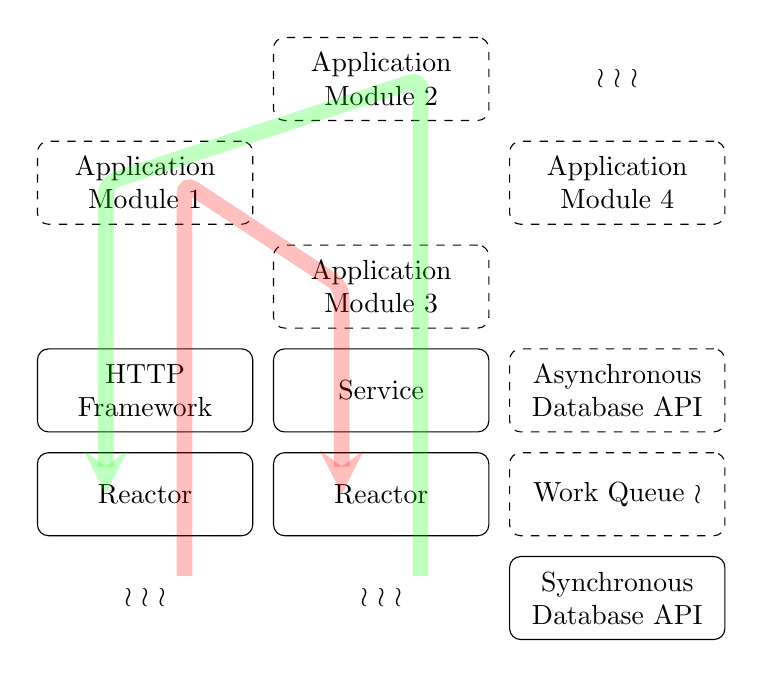
\begin{tikzpicture}
          [ ampersand replacement=\&,
            element/.style={
              rectangle,
              draw,
              rounded corners,
              text width=2.5cm,
              minimum height=3em,
              text centered},
            line/.style={
              draw,
              thick,
              ->,
              >=stealth,
              line width=2mm,
              opacity=.25,
              rounded corners,
            },
          ]

          \matrix [row sep=.25cm, column sep=.25cm] {
            \&
            \node (apm2) [element, dashed] {Application Module 2}; \&
            \node {$\wr$ $\wr$ $\wr$}; \\

            \node (apm1) [element, dashed] {Application Module 1}; \&
            \&
            \node [element, dashed] {Application Module 4}; \\

            \&
            \node (apm3) [element, dashed] {Application Module 3}; \&
            \\

            \node (http) [element] {HTTP Framework}; \&
            \node (service) [element] {Service}; \&
            \node [element, dashed] {Asynchronous Database API}; \\

            \node (reactor1) [element] {Reactor}; \&
            \node (reactor2) [element] {Reactor}; \&
            \node [element, dashed] {Work Queue $\wr$}; \\

            \node (thread1) {$\wr$ $\wr$ $\wr$}; \&
            \node (thread2) {$\wr$ $\wr$ $\wr$}; \&
            \node [element] {Synchronous Database API}; \\
          };

          \draw[line,red] ($(thread1.north) + (.5,0)$) -- ($(reactor1.center) + (.5,0)$) -- ($(http.center) + (.5,0)$) -- ($(apm1.center) + (.5,0)$) -- ($(apm3.center) - (.5,0)$) -- ($(service.center) - (.5,0)$) -- ($(reactor2.center) - (.5,0)$);

          \draw[line,green] ($(thread2.north) + (.5,0)$) -- ($(service.center) + (.5,0)$) -- ($(apm3.center) + (.5,0)$) -- ($(apm2.center) + (.5,0)$) -- ($(apm1.center) + (-.5,0)$) -- ($(http.center) - (.5,0)$) -- ($(reactor1.center) - (.5,0)$);

        \end{tikzpicture}
      }
    \end{column}

    \begin{column}{.4\textwidth}
      \begin{block}{Hazards}
        \begin{itemize}
          \item deadlock
          \item livelock
          \item memory corruption
        \end{itemize}
      \end{block}
      \begin{block}{Brittle unless developers}
        \begin{itemize}
        \item identify and protect shared state
        \item understand call graph
        \item write reactive ``glue code''
        \end{itemize}
      \end{block}

    \end{column}
  \end{columns}

\end{frame}

\begin{frame}{Challenges}
  \centering

  \begin{block}{Reduce Accidental Complexity}
    \begin{itemize}
    \item eliminate shared state
    \item implicit atomicity
    \end{itemize}
  \end{block}

  \begin{block}{Achieve Principled Composition}
    \begin{itemize}
    \item Units and means of composition
    \item ``Well-formed-ness''
    \item Encapsulation
    \item Interface
    \item \emph{Compositionality}
    \item \emph{Substitutional Equivalence}
    \end{itemize}
  \end{block}
\end{frame}

\begin{frame}{Achieve Principled Composition}

  \begin{columns}
    \begin{column}[T]{.45\textwidth}
      \begin{block}{Compositionality}
        $f(x) \mod 2 = 1$ (odd)

        $g(x) \mod 2 = 1$ (odd)

        $h(x) = f(x) + g(x)$

        $h(x) \mod 2 = ?$
      \end{block}
    \end{column}
    \begin{column}[T]{.45\textwidth}
      \begin{block}{Substitutional Equivalence}
        $f(x) = 2x$

        $g(x) = x+1$

        $h(x) = f(g(x)) = 2(x+1)$

        $h(x) = 2x + 2$
      \end{block}
    \end{column}
  \end{columns}

  \vspace*{24pt}

  \begin{center}
    \LARGE
    Straightforward for simple algebras.  How can we achieve this in reactive systems?
  \end{center}

\end{frame}

\begin{frame}{Related Work}

  Abstract Models for Analysis
  \begin{itemize}
  \item e.g., Calculus of Communicating Systems, Algebra of Communicating Processes
  \item Not practical for design and implementation
  \end{itemize}

  Processes-Oriented Models
  \begin{itemize}
  \item e.g., Cooperating Sequential Processes, Communicating Sequential Processes, Kahn Process Networks
  \item Difficult to rewrite $N$ processes as one process
  \end{itemize}

  Asynchronous Message Passing
  \begin{itemize}
  \item e.g., Actor Model
  \item Weak guarantees limit compositional design and reasoning
  \end{itemize}
\end{frame}

\begin{frame}{Related Work}
  UNITY
  \begin{itemize}
  \item State variables, assignment statements, non-deterministic execution
  \item Lack of encapsulation/interface precludes compositionality
  \end{itemize}

  I/O Automata
  \begin{itemize}
  \item State variables, pre/post conditions, signatures (interfaces)
  \item Composition limited in depth, no third-party composition
  \end{itemize}

\end{frame}

\begin{frame}[fragile]{Approach and Contributions}
  \centering
  \begin{tabular}{|C{.4\textwidth}|C{.4\textwidth}|}
    \hline
     \emph{Reactive Components} \newline \emph{Formal Model} & \rcgo{} \newline Programming Language \\

        \resizebox{.25\textwidth}{!}{%
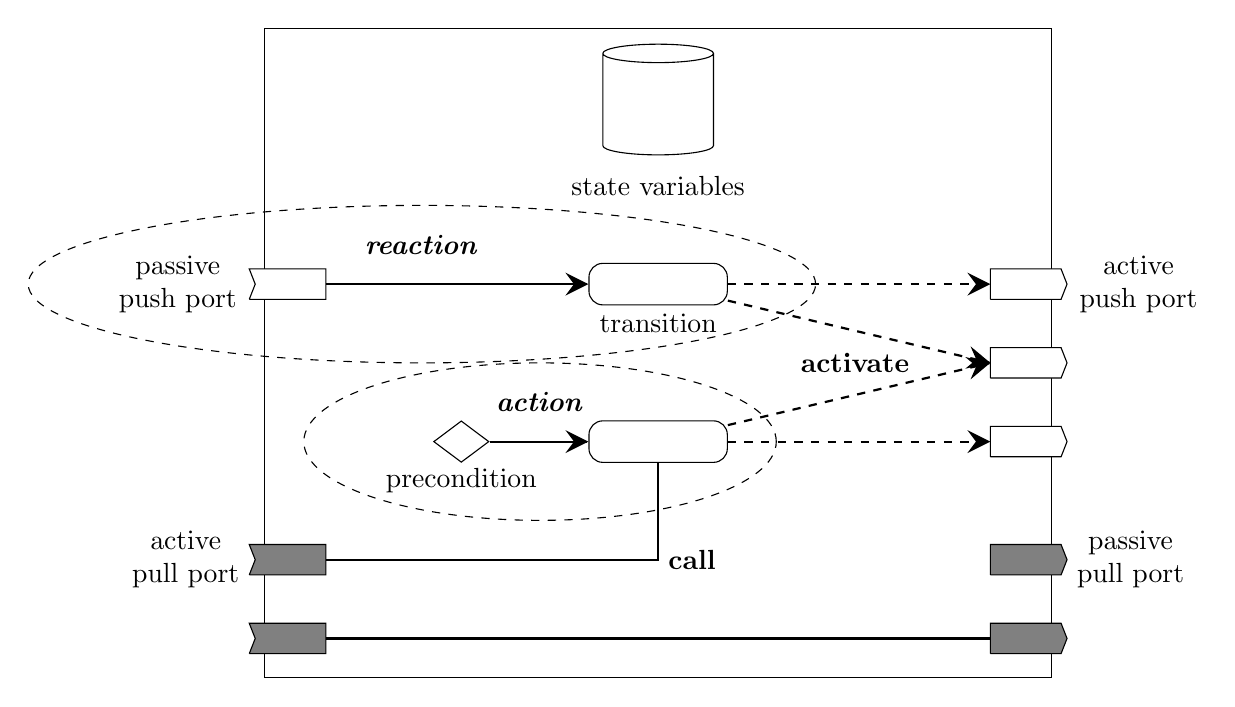
\begin{tikzpicture}
[
arrowstyle/.style={
  decoration={markings,mark=at position 1 with {\arrow[scale=2,]{stealth}}},
  postaction={decorate},
  shorten >=0.4pt
}
]

%% component boundary
\draw (0,0) rectangle (10,8.25);
%% active pull ports
\node (apull1) [shape=leftin, draw, text=gray, fill=gray] at (0,1.5) {man};
\node [align=center] at (-1,1.5) {active\\pull port};
\node (apull2) [shape=leftin, draw, text=gray, fill=gray] at (0,.5) {man};
%% passive pull ports
\node (ppull1) [shape=rightout, draw, text=gray, fill=gray] at (10, 1.5) {man};
\node [align=center] at (11,1.5) {passive\\pull port};
\node (ppull2) [shape=rightout, draw, text=gray, fill=gray] at (10, .5) {man};
\draw [thick] (apull2.east) -- (ppull2.west);
%% actions and reactions
\node [draw, diamond, minimum height=15, minimum width=20] (pre) at (2.5,3) {};
\node at (2.5,2.5) {precondition};
\node [draw, minimum height=15, minimum width=50, rounded corners=5] (trans1) at (5,3) {};
\draw [dashed] (3.5,3) ellipse (3 and 1);
\node at (3.5,3.5) {\textbf{\emph{action}}};
\node [draw, minimum height=15, minimum width=50, rounded corners=5] (trans2) at (5,5) {};
\node at (5,4.5) {transition};
\draw [thick,arrowstyle] (pre) -- (trans1);
\draw [thick] (apull1.east) -| (trans1) node[pos=.5,right] {\textbf{call}};
%% active push ports
\node (apush1) [shape=rightout, draw, text=white, fill=white] at (10, 3) {man};
\node (apush2) [shape=rightout, draw, text=white, fill=white] at (10, 4) {man};
\node (apush3) [shape=rightout, draw, text=white, fill=white] at (10, 5) {man};
\node [align=center] at (11.1,5) {active\\push port};
\draw [thick,dashed,arrowstyle] (trans1) -- (apush1.west);
\draw [thick,dashed,arrowstyle] (trans1) -- (apush2.west);
\node at(7.5,4) {\textbf{activate}};
\draw [thick,dashed,arrowstyle] (trans2) -- (apush2.west);
\draw [thick,dashed,arrowstyle] (trans2) -- (apush3.west);
%% passive push ports
\node (ppush1) [shape=leftin, draw, text=white, fill=white] at (0, 5) {man};
\draw [thick,arrowstyle] (ppush1.east) -- (trans2);
\node [align=center] at (-1.1,5) {passive\\push port};
\draw [dashed] (2,5) ellipse (5 and 1);
\node at (2,5.5) {\textbf{\emph{reaction}}};
\node [draw, cylinder, shape border rotate=90, minimum height=40, minimum width=40] (sv1) at (5,7.25) {};
\node [align=center] at (5,6.25) {state variables};
\end{tikzpicture}
}%
        &
        {\center
\lstset{
  language={rcgo},
  basicstyle=\tiny\ttfamily,
  columns=fixed,
}

\begin{lstlisting}
type Clock component {
  counter uint;
  flag bool;
  response push (t uint);
};
...
\end{lstlisting}
}

        \\
        \hline
        \rcgo{} Platform & \rcgo{} Scheduler \\

\begin{center}
\resizebox{.25\textwidth}{!}{%
\begingroup
\fontsize{10pt}{12pt}\selectfont
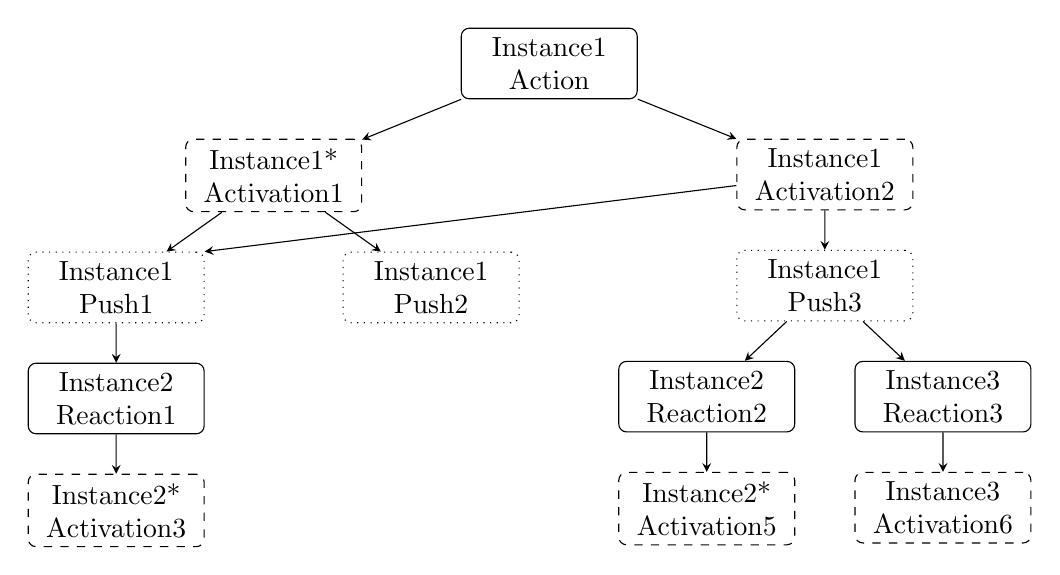
\begin{tikzpicture}[
    arrowstyle/.style={draw, -stealth},
    edge from parent/.style={draw, -stealth},
    reaction/.style={rectangle, draw, rounded corners=1mm, text width=2cm,
        text centered, anchor=north},
    activation/.style={rectangle, draw, rounded corners=1mm, dashed, text width=2cm,
        text centered, anchor=north},
    push/.style={rectangle, draw, rounded corners=1mm, dotted, text width=2cm,
        text centered, anchor=north},
    level 1/.style={sibling distance=7.0cm},
    level 2/.style={sibling distance=4.0cm},
    level 3/.style={sibling distance=3.0cm},
    level distance=0.5cm, growth parent anchor=south
]
\node (Action) [reaction] {Instance1 Action}
  child {
    node (Activation01) [activation] {Instance1* Activation1}
    child {
      node (Push01) [push] {Instance1 Push1}
      child {
        node (Reaction01) [reaction] {Instance2 Reaction1}
        child {
          node (Activation03) [activation] {Instance2* Activation3}
        }
      }
    }
    child {
      node (Push02) [push] {Instance1 Push2}
    }
  }
  child {
    node (Activation02) [activation] {Instance1 Activation2}
    child {
      node (Push03) [push] {Instance1 Push3}
      child {
        node (Reaction02) [reaction] {Instance2 Reaction2}
        child {
          node (Activation04) [activation] {Instance2* Activation5}
        }
      }
      child {
        node (Reaction03) [reaction] {Instance3 Reaction3}
        child {
          node (Activation05) [activation] {Instance3 Activation6}
        }
      }
    }
  }
;

\draw[arrowstyle] (Activation02) -- (Push01.north east);

\end{tikzpicture}
\endgroup
}%
\end{center}
&
\includegraphics[width=.25\textwidth]{async_throughput_box.png}
\\
        \hline
  \end{tabular}


\end{frame}

\begin{frame}{Reactive Components Model}
  \centering

        \resizebox{\textwidth}{!}{%
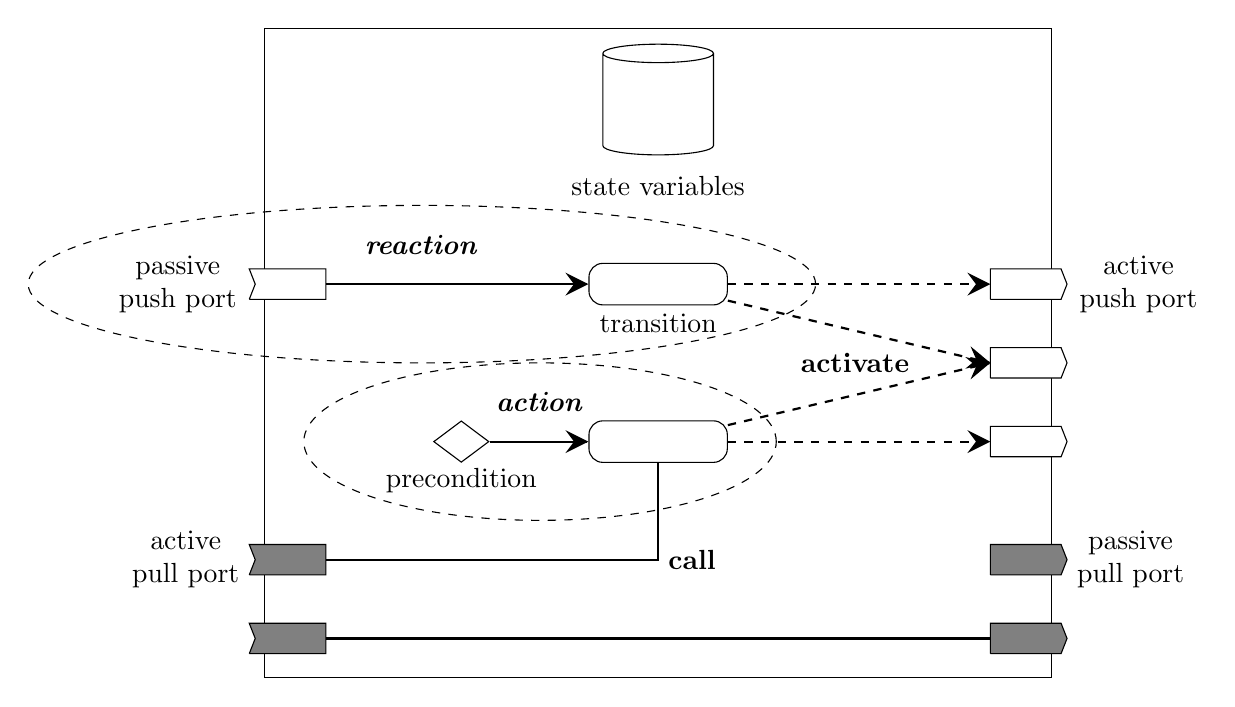
\begin{tikzpicture}
[
arrowstyle/.style={
  decoration={markings,mark=at position 1 with {\arrow[scale=2,]{stealth}}},
  postaction={decorate},
  shorten >=0.4pt
}
]

%% component boundary
\draw (0,0) rectangle (10,8.25);
%% active pull ports
\node (apull1) [shape=leftin, draw, text=gray, fill=gray] at (0,1.5) {man};
\node [align=center] at (-1,1.5) {active\\pull port};
\node (apull2) [shape=leftin, draw, text=gray, fill=gray] at (0,.5) {man};
%% passive pull ports
\node (ppull1) [shape=rightout, draw, text=gray, fill=gray] at (10, 1.5) {man};
\node [align=center] at (11,1.5) {passive\\pull port};
\node (ppull2) [shape=rightout, draw, text=gray, fill=gray] at (10, .5) {man};
\draw [thick] (apull2.east) -- (ppull2.west);
%% actions and reactions
\node [draw, diamond, minimum height=15, minimum width=20] (pre) at (2.5,3) {};
\node at (2.5,2.5) {precondition};
\node [draw, minimum height=15, minimum width=50, rounded corners=5] (trans1) at (5,3) {};
\draw [dashed] (3.5,3) ellipse (3 and 1);
\node at (3.5,3.5) {\textbf{\emph{action}}};
\node [draw, minimum height=15, minimum width=50, rounded corners=5] (trans2) at (5,5) {};
\node at (5,4.5) {transition};
\draw [thick,arrowstyle] (pre) -- (trans1);
\draw [thick] (apull1.east) -| (trans1) node[pos=.5,right] {\textbf{call}};
%% active push ports
\node (apush1) [shape=rightout, draw, text=white, fill=white] at (10, 3) {man};
\node (apush2) [shape=rightout, draw, text=white, fill=white] at (10, 4) {man};
\node (apush3) [shape=rightout, draw, text=white, fill=white] at (10, 5) {man};
\node [align=center] at (11.1,5) {active\\push port};
\draw [thick,dashed,arrowstyle] (trans1) -- (apush1.west);
\draw [thick,dashed,arrowstyle] (trans1) -- (apush2.west);
\node at(7.5,4) {\textbf{activate}};
\draw [thick,dashed,arrowstyle] (trans2) -- (apush2.west);
\draw [thick,dashed,arrowstyle] (trans2) -- (apush3.west);
%% passive push ports
\node (ppush1) [shape=leftin, draw, text=white, fill=white] at (0, 5) {man};
\draw [thick,arrowstyle] (ppush1.east) -- (trans2);
\node [align=center] at (-1.1,5) {passive\\push port};
\draw [dashed] (2,5) ellipse (5 and 1);
\node at (2,5.5) {\textbf{\emph{reaction}}};
\node [draw, cylinder, shape border rotate=90, minimum height=40, minimum width=40] (sv1) at (5,7.25) {};
\node [align=center] at (5,6.25) {state variables};
\end{tikzpicture}
}%
\end{frame}

\begin{frame}{Clock System Example \includegraphics[height=12pt]{CLOCK01-300px.png}}

\centering
\resizebox{\textwidth}{!}{%
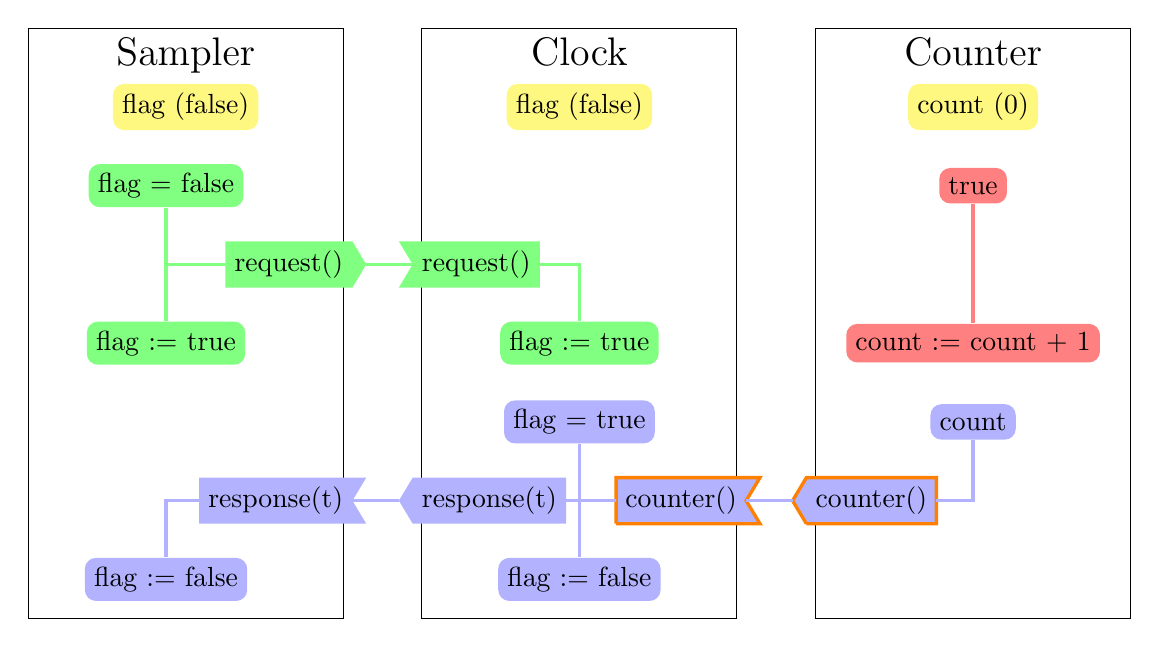
\begin{tikzpicture}
  [
    initial/.style={
      fill=yellow!50,
      rounded corners,
    },
    trans1/.style={
      fill=green!50,
    },
    trans1line/.style={
      draw=green!50,
    },
    trans2/.style={
      fill=blue!30,
    },
    trans2line/.style={
      draw=blue!30,
    },
    trans3/.style={
      fill=red!50,
    },
    trans3line/.style={
      draw=red!50,
    },
    line/.style={
      very thick
    },
    pre/.style={
      rectangle,
      rounded corners
    },
    post/.style={
      rectangle,
      rounded corners
    },
    pull/.style={
      draw=orange, very thick
    }
  ]
% Sampler
\draw (2,2.5) rectangle (6,10);
\node [below] at (4,10) {\Large Sampler};
\node [initial] at (4,9) {flag (false)};

\node (pre1)  [trans1, pre]            at (3.75,8) {flag = false};
\node (ex2a)  [trans1, shape=rightout] at (6,7)    {request()};
\node (post1) [trans1, post]           at (3.75,6) {flag := true};
\draw [trans1line, line] (pre1.south) |- (ex2a.west) -| (post1.north);

\node (ex3a)  [trans2, shape=rightin]  at (6,4)    {response(t)};
\node (post2) [trans2, post]           at (3.75,3) {flag := false};
\draw [trans2line, line] (ex3a.west) -| (post2.north);

% Clock
\draw (7,2.5) rectangle (11,10);
\node [below] at (9,10) {\Large Clock};
\node [initial] at (9,9) {flag (false)};

\node (ex2b)  [trans1, shape=leftin] at (7,7) {request()};
\node (post2) [trans1, post]         at (9,6) {flag := true};
\draw [trans1line, line] (ex2b.east) -| (post2.north);

\node (pre2)  [trans2, pre]           at (9,5)  {flag = true};
\node (ex3b)  [trans2, shape=leftout] at (7,4)  {response(t)};
\node (pull)  [trans2, shape=rightin, pull] at (11,4) {counter()};
\node (post3) [trans2, post]          at (9,3)  {flag := false};
\draw [trans2line, line] (pre2.south) |- (ex3b.east) -| (pull.west) -| (post3.north);

% Counter
\draw (12,2.5) rectangle (16,10);
\node [below] at (14,10) {\Large Counter};
\node [initial] at (14,9) {count (0)};

\node (pre4)  [trans3, pre]  at (14,8) {true};
\node (post4) [trans3, post] at (14,6) {count := count + 1};
\draw [trans3line, line] (pre4.south) -- (post4.north);

\node (pre3)   [trans2, pre]           at (14,5) {count};
\node (getter) [trans2, shape=leftout, pull] at (12,4) {counter()};
\draw [trans2line, line] (pre3.south) |- (getter.east);

\draw [trans1line, line] (ex2a.east) -- (ex2b.west);
\draw [trans2line, line] (ex3a.east) -- (ex3b.west);
\draw [trans2line, line] (pull.east) -- (getter.west);

\end{tikzpicture}
}%

\end{frame}

\begin{frame}{Simplification of Clock System \includegraphics[height=12pt]{CLOCK01-300px.png}}

  \centering

  Reactive components allow composition.

\resizebox{\textwidth}{!}{%
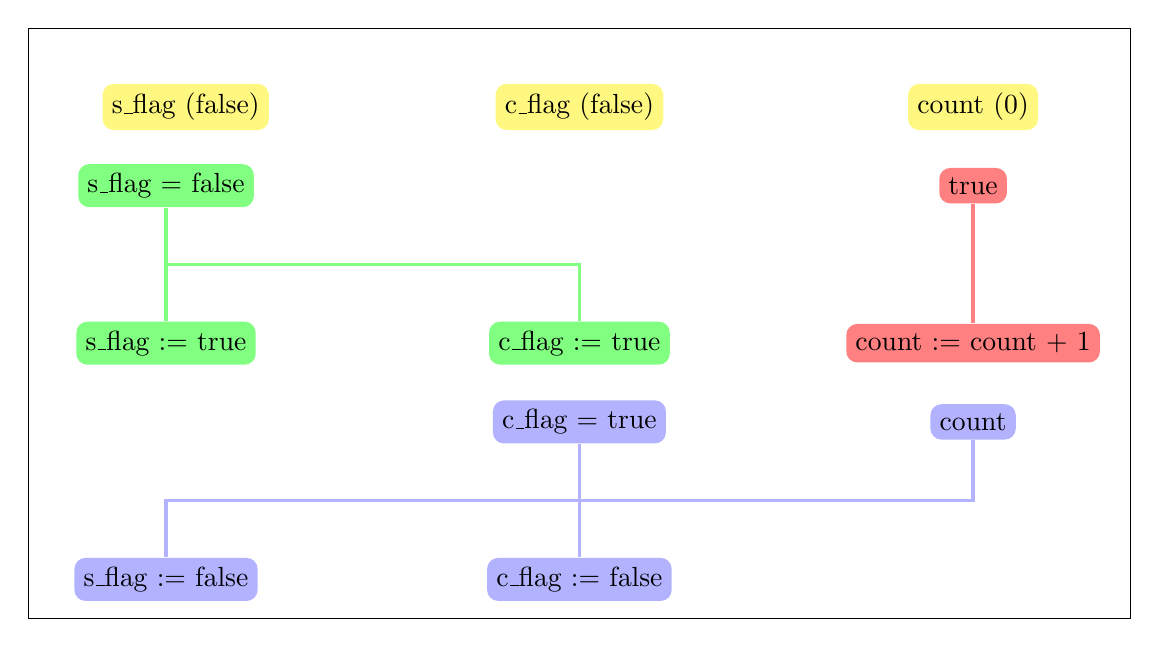
\begin{tikzpicture}
  [
    initial/.style={
      fill=yellow!50,
      rounded corners,
    },
    trans1/.style={
      fill=green!50,
    },
    trans1line/.style={
      draw=green!50,
    },
    trans2/.style={
      fill=blue!30,
    },
    trans2line/.style={
      draw=blue!30,
    },
    trans3/.style={
      fill=red!50,
    },
    trans3line/.style={
      draw=red!50,
    },
    line/.style={
      very thick
    },
    pre/.style={
      rectangle,
      rounded corners
    },
    post/.style={
      rectangle,
      rounded corners
    },
    pull/.style={
      draw=orange, very thick
    }
  ]
% Sampler
\draw (2,2.5) rectangle (16,10);
\node [initial] at (4,9) {s\_flag (false)};

\node (pre1)  [trans1, pre]            at (3.75,8) {s\_flag = false};
\node (post1) [trans1, post]           at (3.75,6) {s\_flag := true};
\draw [trans1line, line] (pre1.south) |- (6,7) -| (post1.north);

\node (post2) [trans2, post]           at (3.75,3) {s\_flag := false};
\draw [trans2line, line] (6,4) -| (post2.north);

% Clock
\node [initial] at (9,9) {c\_flag (false)};

\node (post2) [trans1, post]         at (9,6) {c\_flag := true};
\draw [trans1line, line] (7,7) -| (post2.north);

\node (pre2)  [trans2, pre]           at (9,5)  {c\_flag = true};
\node (post3) [trans2, post]          at (9,3)  {c\_flag := false};
\draw [trans2line, line] (pre2.south) |- (7,4) -| (11,4) -| (post3.north);

% Counter
\node [initial] at (14,9) {count (0)};

\node (pre4)  [trans3, pre]  at (14,8) {true};
\node (post4) [trans3, post] at (14,6) {count := count + 1};
\draw [trans3line, line] (pre4.south) -- (post4.north);

\node (pre3)   [trans2, pre]           at (14,5) {count};
\draw [trans2line, line] (pre3.south) |- (12,4);

\draw [trans1line, line] (6,7) -- (7,7);
\draw [trans2line, line] (6,4) -- (7,4);
\draw [trans2line, line] (11,4) -- (12,4);

\end{tikzpicture}
}%

\end{frame}

\begin{frame}{Platform Requirements}
  \begin{center}
  \begin{tikzpicture}
    [
      ampersand replacement=\&,
      node distance=5cm,
      node/.style={
        rectangle,
        draw,
        rounded corners,
        minimum height=3em,
        text width=2cm,
        text centered,
        very thick
      },
      line/.style = {
        >=stealth,
        ->,
        very thick,
      }
    ]

    \matrix [row sep=.25cm, column sep=1cm] {
      \node (m) [node] {Model}; \&
      \node (p) [node] {Platform}; \&
      \node (s) [node] {Systems}; \\
    };

    \node at ($(m.south east)!.5!(p.south west)$) {\includegraphics[height=.75cm]{thumbs.png}};
    \node at ($(p.south east)!.5!(s.south west)$) {\includegraphics[height=.75cm]{thumbs.png}};

    \draw[line] ($(m.south east)!.66!(m.north east)$) -- ($(p.south west)!.66!(p.north west)$);
    \draw[line] ($(p.south east)!.66!(p.north east)$) -- ($(s.south west)!.66!(s.north west)$);
    \draw[line] ($(s.south west)!.33!(s.north west)$) -- ($(p.south east)!.33!(p.north east)$);
    \draw[line] ($(p.south west)!.33!(p.north west)$) -- ($(m.south east)!.33!(m.north east)$);
  \end{tikzpicture}
  \end{center}

  \vspace*{-20pt}

  \begin{center}
  \begin{columns}
    \begin{column}{.25\textwidth}
      \center
      \includegraphics[width=3cm]{mind_the_gap_edit.png}
    \end{column}
    \begin{column}{.75\textwidth}
      \center
      \begin{itemize}
      \item Strict enforcement of the model
      \item Reference semantics and linked data structures
      \item Efficient inter-component communication
      \end{itemize}
    \end{column}
  \end{columns}
  \end{center}

  \vspace*{-20pt}

  \begin{columns}
    \begin{column}{.5\textwidth}
      \fbox{
        \parbox{\linewidth}{\raggedright
          \emph{Static System Assumption}:\\Number and configuration of components is fixed.
        }
      }
    \end{column}
    \begin{column}{.5\textwidth}
      \begin{itemize}
      \item \rcgo{} is based on Go \includegraphics[height=32pt]{gopher.png}
      \item C with methods, interfaces, and garbage collection
      \item rc\textsubscript{java} would be different
      \end{itemize}
    \end{column}
  \end{columns}


\end{frame}

\begin{frame}[fragile]{\rcgo{}:  Keywords}

{\small
\begin{lstlisting}
type Clock component {
  counter uint;
  flag bool;
  response push (t uint);
  counter pull () uint;
};

init (c *Clock) Initialize () {.}
action (c $const *Clock) Respond (this.flag) {.}
reaction (c $const *Clock) Request () {.}
getter (c $const *Counter) Counter () uint {.}

bind (s *System) BindAll {
  s.sampler.Request -> s.clock.Request;
  s.clock.counter   <- s.counter.Counter;
}

instance s System Initialize ();
\end{lstlisting}
}

\onslide<2->
\begin{tikzpicture}[overlay,remember picture]
  \pgftransformshift{\pgfpointanchor{current page}{center}}
  \node [draw, cylinder, shape border rotate=90, minimum height=20, minimum width=20, fill=white] (sv1) at (-1.5,2.75) {};
\end{tikzpicture}

\onslide<3->
\begin{tikzpicture}[overlay,remember picture]
  \pgftransformshift{\pgfpointanchor{current page}{center}}
  \node [shape=rightout, draw, text=white, fill=white] at (1, 2.3) {man};
\end{tikzpicture}

\onslide<4->
\begin{tikzpicture}[overlay,remember picture]
  \pgftransformshift{\pgfpointanchor{current page}{center}}
  \node [shape=leftin, draw, text=gray, fill=gray] at (.4,1.8) {man};
\end{tikzpicture}

\onslide<5->
\begin{tikzpicture}[overlay,remember picture]
  \pgftransformshift{\pgfpointanchor{current page}{center}}
  \node [draw, diamond, minimum height=15, minimum width=20, fill=white] at (3.1,.5) {};
  \node [draw, minimum height=15, minimum width=20, rounded corners=5, fill=white] at (4.88,.6) {};
\end{tikzpicture}

\onslide<6->
\begin{tikzpicture}[overlay,remember picture]
  \pgftransformshift{\pgfpointanchor{current page}{center}}
  \node [shape=leftin, draw, text=white, fill=white] at (4,-.25) {man};
\end{tikzpicture}

\onslide<7->
\begin{tikzpicture}[overlay,remember picture]
  \pgftransformshift{\pgfpointanchor{current page}{center}}
  \node [shape=rightout, draw, text=gray, fill=gray] at (6, -.7) {man};
\end{tikzpicture}

\onslide<8->
\begin{tikzpicture}[overlay,remember picture]
  \pgftransformshift{\pgfpointanchor{current page}{center}}
  \draw[thick] (4,-2.1) -- (6,-2.1);
\end{tikzpicture}

\onslide<9->
\begin{tikzpicture}[overlay,remember picture]
  \pgftransformshift{\pgfpointanchor{current page}{center}}
  \node [rectangle, draw, minimum height=15, minimum width=20, fill=white] at (2.1, -3.625) {};
\end{tikzpicture}

\end{frame}

\begin{frame}[fragile]{\rcgo{}:  Activations}

\begin{lstlisting}
action (this $const *QueueProcessor) _dequeue
(!this.queue.Empty()) {

  var m $const *MetaData =
    this.lookupMetadata(this.queue.Front())

  activate Out (this.queue.Front(), m) {
    this.queue.Pop()
  }

}
\end{lstlisting}

\onslide<2>
\begin{tikzpicture}[overlay,remember picture]
  \pgftransformshift{\pgfpointanchor{current page}{center}}
  \node[
    rectangle callout,
    draw=eclipseGreen,
    ultra thick,
    fill=white,
    decorate,
    callout absolute pointer={(-.75,1.75)},
    font=\Large,
    text width=0.6\textwidth,
    align=center,
    anchor=center
  ] at (2.5,-3) {actions/reactions start in immutable phase};
\end{tikzpicture}

\onslide<3>
\begin{tikzpicture}[overlay,remember picture]
  \pgftransformshift{\pgfpointanchor{current page}{center}}
  \node[
    rectangle callout,
    draw=eclipseGreen,
    ultra thick,
    fill=white,
    decorate,
    callout absolute pointer={(-.75,-.25)},
    font=\Large,
    text width=0.6\textwidth,
    align=center,
    anchor=center
  ] at (2.5,-3) {activate bodies are in mutable phase};
\end{tikzpicture}

\onslide<4>
\begin{tikzpicture}[overlay,remember picture]
  \pgftransformshift{\pgfpointanchor{current page}{center}}
  \node[
    rectangle callout,
    draw=eclipseGreen,
    ultra thick,
    fill=white,
    decorate,
    callout absolute pointer={(-4.8,-1.1)},
    font=\Large,
    text width=0.6\textwidth,
    align=center,
    anchor=center
  ] at (2.5,-3) {activate terminates action/reaction};
\end{tikzpicture}

\end{frame}

\begin{frame}[fragile]{\rcgo{}:  Reference Semantics}

\begin{lstlisting}
reaction (this $const *C) R (w *W) {
  if (interesting(w)) {
    activate {
      this.w = w // Save for later
    }}}
\end{lstlisting}

\vspace*{-8pt}

\begin{columns}
  \begin{column}{.5\textwidth}
\begin{center}
  Compositionality is lost!
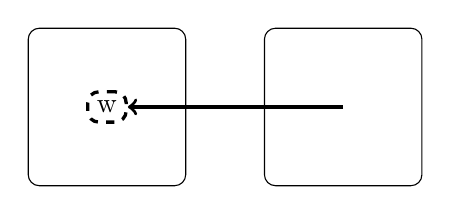
\begin{tikzpicture}
  [object/.style={
      draw=black, very thick,
      dashed,
      rounded corners,
      text centered,
    },
    component/.style={
      rounded corners
    }
  ]
  \draw[component] (0,0) rectangle (2,2);
  \draw[component] (3,0) rectangle (5,2);
  \node[object] (w) at (1,1) {w};
  \draw[->, very thick] (4,1) -> (w.east);
\end{tikzpicture}
\end{center}
  \end{column}
  \begin{column}{.5\textwidth}
    \begin{block}{Safe Reference Semantics}
      \begin{itemize}
      \item component state is private
      \item \verb+$foreign+ attribute for pointers (read, \sout{write}, \sout{save})
      %%\item ports, reactions, getters, and initializers must be \emph{foreign safe}
      \end{itemize}
    \end{block}
  \end{column}
\end{columns}

\begin{lstlisting}
reaction (this $const *C) R (w $foreign *W) {
  if (interesting(w)) {
    var w2 *W = w.DeepCopy()
    activate {
      this.w = w2 // Save for later
    }}}
\end{lstlisting}

\end{frame}

\begin{frame}[fragile]{\rcgo{}:  Move Semantics}

\begin{lstlisting}
action (this $const *C1) A (precondition) {
  var w *heap W = new(heap W)
  change (w, x) {
    x.foo = 3
    ...
  }
  activate port (w) {
    ...
  }}

reaction (this $const *C2) R (w $foreign *heap W) {
  var y *heap W = move(w)
  // Or
  var z *W = merge(w)
  ...
}
\end{lstlisting}

\onslide<2>
\begin{tikzpicture}[overlay,remember picture]
  \pgftransformshift{\pgfpointanchor{current page}{center}}
  \node[
    rectangle callout,
    draw=eclipseGreen,
    ultra thick,
    fill=white,
    decorate,
    callout absolute pointer={(-1,2.9)},
    font=\Large,
    text width=0.6\textwidth,
    align=center,
    anchor=center
  ] at (2.5,0) {allocate a new heap};
\end{tikzpicture}

\onslide<3>
\begin{tikzpicture}[overlay,remember picture]
  \pgftransformshift{\pgfpointanchor{current page}{center}}
  \node[
    rectangle callout,
    draw=eclipseGreen,
    ultra thick,
    fill=white,
    decorate,
    callout absolute pointer={(-2.2,2.5)},
    font=\Large,
    text width=0.6\textwidth,
    align=center,
    anchor=center
  ] at (2.5,0) {x is a *W};
\end{tikzpicture}

\onslide<4>
\begin{tikzpicture}[overlay,remember picture]
  \pgftransformshift{\pgfpointanchor{current page}{center}}
  \node[
    rectangle callout,
    draw=eclipseGreen,
    ultra thick,
    fill=white,
    decorate,
    callout absolute pointer={(-2.2,2.3)},
    font=\Large,
    text width=0.6\textwidth,
    align=center,
    anchor=center
  ] at (2.5,0) {all variables outside of \verb+change+ are \verb+foreign+};
\end{tikzpicture}

\onslide<5>
\begin{tikzpicture}[overlay,remember picture]
  \pgftransformshift{\pgfpointanchor{current page}{center}}
  \node[
    rectangle callout,
    draw=eclipseGreen,
    ultra thick,
    fill=white,
    decorate,
    callout absolute pointer={(-1,-1)},
    font=\Large,
    text width=0.6\textwidth,
    align=center,
    anchor=center
  ] at (2.5,0) {take ownership};
\end{tikzpicture}

\onslide<6>
\begin{tikzpicture}[overlay,remember picture]
  \pgftransformshift{\pgfpointanchor{current page}{center}}
  \node[
    rectangle callout,
    draw=eclipseGreen,
    ultra thick,
    fill=white,
    decorate,
    callout absolute pointer={(-1.8,-1.8)},
    font=\Large,
    text width=0.6\textwidth,
    align=center,
    anchor=center
  ] at (2.5,0) {take ownership and unbox};
\end{tikzpicture}

\onslide<7>
\begin{tikzpicture}[overlay,remember picture]
  \pgftransformshift{\pgfpointanchor{current page}{center}}
  \node[
    rectangle callout,
    draw=eclipseGreen,
    ultra thick,
    fill=white,
    decorate,
    callout absolute pointer={(-3.5,.5)},
    font=\Large,
    text width=0.6\textwidth,
    align=center,
    anchor=center
  ] at (2.5,0) {content behind w is gone};
\end{tikzpicture}

\end{frame}

\begin{frame}{Enforcing Sound Composition:  The Transaction Graph}

  \centering

  \begin{description}
  \item[Transaction Graph] follow activations through code and bindings
  \end{description}

  Action/Reaction $\to$ Activation $\to$ Port $\to$ Reaction $\to$ \ldots

  \resizebox{.9\textwidth}{!}{
  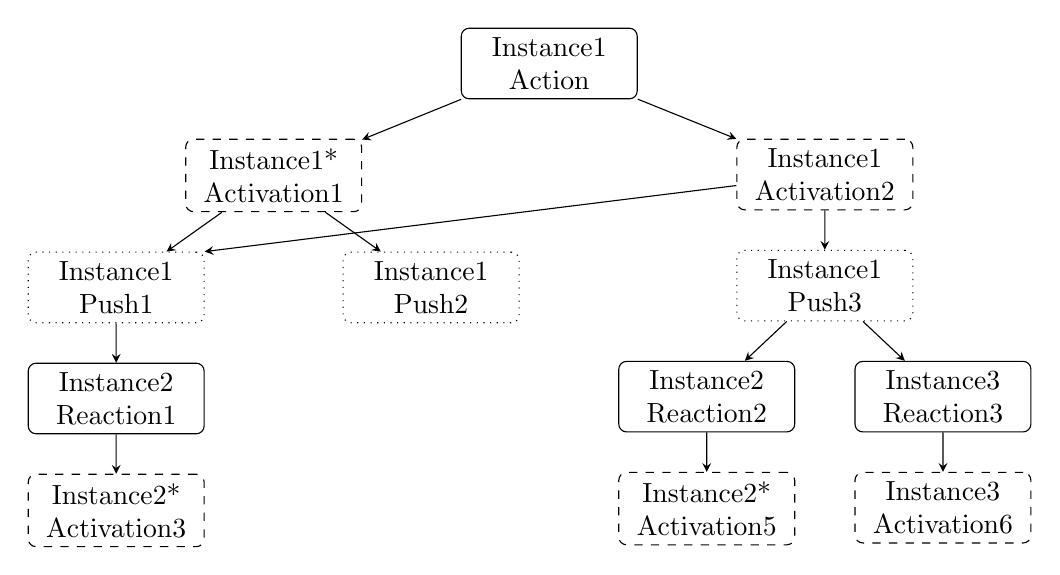
\begin{tikzpicture}[
    arrowstyle/.style={draw, -stealth},
    edge from parent/.style={draw, -stealth},
    reaction/.style={rectangle, draw, rounded corners=1mm, text width=2cm,
        text centered, anchor=north},
    activation/.style={rectangle, draw, rounded corners=1mm, dashed, text width=2cm,
        text centered, anchor=north},
    push/.style={rectangle, draw, rounded corners=1mm, dotted, text width=2cm,
        text centered, anchor=north},
    level 1/.style={sibling distance=7.0cm},
    level 2/.style={sibling distance=4.0cm},
    level 3/.style={sibling distance=3.0cm},
    level distance=0.5cm, growth parent anchor=south
]
\node (Action) [reaction] {Instance1 Action}
  child {
    node (Activation01) [activation] {Instance1* Activation1}
    child {
      node (Push01) [push] {Instance1 Push1}
      child {
        node (Reaction01) [reaction] {Instance2 Reaction1}
        child {
          node (Activation03) [activation] {Instance2* Activation3}
        }
      }
    }
    child {
      node (Push02) [push] {Instance1 Push2}
    }
  }
  child {
    node (Activation02) [activation] {Instance1 Activation2}
    child {
      node (Push03) [push] {Instance1 Push3}
      child {
        node (Reaction02) [reaction] {Instance2 Reaction2}
        child {
          node (Activation04) [activation] {Instance2* Activation5}
        }
      }
      child {
        node (Reaction03) [reaction] {Instance3 Reaction3}
        child {
          node (Activation05) [activation] {Instance3 Activation6}
        }
      }
    }
  }
;

\draw[arrowstyle] (Activation02) -- (Push01.north east);

\end{tikzpicture}
  }

  * indicates instance is mutated

\end{frame}

\begin{frame}{Enforcing Sound Composition:  Instance Sets}

  \centering

  \begin{description}
  \item[Instance Set] self and union of instances of children
  \end{description}

  \resizebox{.9\textwidth}{!}{
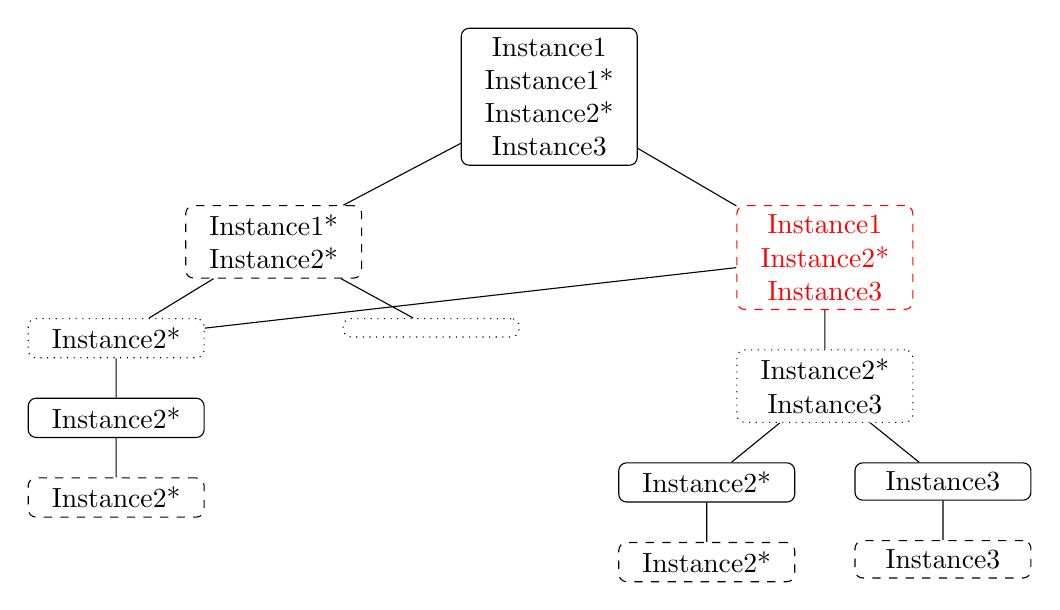
\begin{tikzpicture}[
    reaction/.style={rectangle, draw, rounded corners=1mm, text width=2cm,
        text centered, anchor=north},
    activation/.style={rectangle, draw, rounded corners=1mm, dashed, text width=2cm,
        text centered, anchor=north},
    push/.style={rectangle, draw, rounded corners=1mm, dotted, text width=2cm,
        text centered, anchor=north},
    level 1/.style={sibling distance=7.0cm},
    level 2/.style={sibling distance=4.0cm},
    level 3/.style={sibling distance=3.0cm},
    level distance=0.5cm, growth parent anchor=south
]
\node (Action) [reaction] {Instance1 Instance1* Instance2* Instance3}
  child {
    node (Activation01) [activation] {Instance1* Instance2*}
    child {
      node (Push01) [push] {Instance2*}
      child {
        node (Reaction01) [reaction] {Instance2*}
        child {
          node (Activation03) [activation] {Instance2*}
        }
      }
    }
    child {
      node (Push02) [push] {}
    }
  }
  child {
    node (Activation02) [activation,red] {Instance1 Instance2* Instance3}
    child {
      node (Push03) [push] {Instance2* Instance3}
      child {
        node (Reaction02) [reaction] {Instance2*}
        child {
          node (Activation04) [activation] {Instance2*}
        }
      }
      child {
        node (Reaction03) [reaction] {Instance3}
        child {
          node (Activation05) [activation] {Instance3}
        }
      }
    }
  }
;

\draw (Activation02) -- (Push01);

\end{tikzpicture}
  }

  \begin{itemize}
  \item Activations at same level are \emph{mutually exclusive}
  \item Actions, reactions, and ports are \emph{potentially coincidental}
  \end{itemize}

\onslide<2>
\begin{tikzpicture}[overlay,remember picture]
  \pgftransformshift{\pgfpointanchor{current page}{center}}
  \node[
    ellipse,
    draw=red,
    thick,
    decorate,
    align=center,
    anchor=center,
    minimum width=2.2cm
  ] at (2.8,.6) {};
\end{tikzpicture}

\end{frame}

\begin{frame}{Synchronized Two-Phase Calling Convention}

  \begin{columns}
    \begin{column}{.4\textwidth}
      To execute a transaction:
      \begin{enumerate}
      \item Depth-first traversal of transaction graph (immutable phase)
      \item Execute continuation of activate statements (mutable phase)
      \end{enumerate}
      \vspace*{12pt}
      \emph{Maps well to existing architectures!}
    \end{column}
    \begin{column}{.6\textwidth}
  \resizebox{!}{.7\textheight}{%
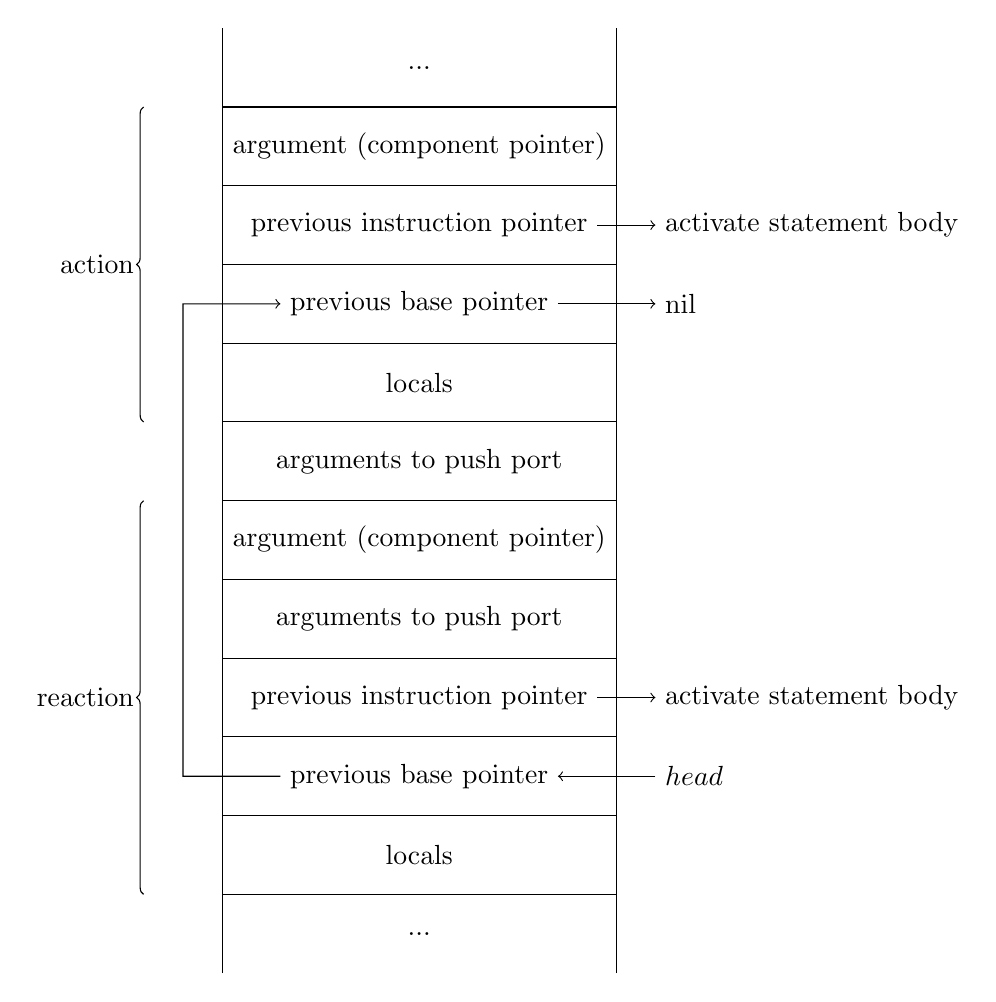
\begin{tikzpicture}
%% component boundary

\draw (0,-5) -- (0,7);
\draw (5,-5) -- (5,7);

\node at (2.5, 6.5) { ... };
\draw (0,6) -- (5,6);
\node at (2.5, 5.5) { argument (component pointer) };
\draw (0,5) -- (5,5);
\node (pip1) at (2.5, 4.5) { previous instruction pointer };
\draw (0,4) -- (5,4);
\node (pbp1) at (2.5, 3.5) { previous base pointer };
\draw (0,3) -- (5,3);
\node at (2.5, 2.5) { locals };
\draw (0,2) -- (5,2);
\node at (2.5, 1.5) { arguments to push port };
\draw (0,1) -- (5,1);
\node at (2.5, .5) { argument (component pointer) };
\draw (0,0) -- (5,0);
\node at (2.5, -.5) { arguments to push port };
\draw (0,-1) -- (5,-1);
\node (pip2) at (2.5, -1.5) { previous instruction pointer };
\draw (0,-2) -- (5,-2);
\node (pbp2) at (2.5, -2.5) { previous base pointer };
\draw (0,-3) -- (5,-3);
\node at (2.5, -3.5) { locals };
\draw (0,-4) -- (5,-4);
\node at (2.5, -4.5) { ... };

\node[anchor=west] (as1) at (5.5, 4.5) { activate statement body };
\draw[->] (pip1) -- (as1);
\node[anchor=west] (as2) at (5.5, -1.5) { activate statement body };
\draw[->] (pip2) -- (as2);

\draw[->] (pbp2) -- ++(-3,0) -- ++(0,6) -- (pbp1);

\node[anchor=west] (nil) at (5.5, 3.5) { nil };
\draw[->] (pbp1) -- (nil);

\node[anchor=west] (head) at (5.5, -2.5) { $head$ };
\draw[->] (head) -- (pbp2);

\draw[decorate,decoration={brace}] (-1,2) -- (-1,6) node[anchor=east,midway] { action };

\draw[decorate,decoration={brace}] (-1,-4) -- (-1,1) node[anchor=east,midway] { reaction };

\end{tikzpicture}
}%
    \end{column}
  \end{columns}
\end{frame}

\begin{frame}{Heaps}
  \begin{block}{Problem}
    Move state from one component to another efficiently
  \end{block}

  \begin{block}{Challenge}
    Maintain isolation of components (encapsulation)
  \end{block}

\end{frame}

\begin{frame}[fragile]{Heaps:  Approach}

  \begin{columns}

    \begin{column}{.5\textwidth}
      \begin{itemize}
      \item Run-time maintains a stack of heaps
      \item Top heap services allocation requests
      \item \verb+change+ scoping rules enforce encapsulation
      \end{itemize}
    \end{column}

    \begin{column}{.5\textwidth}
      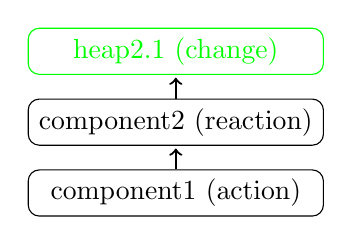
\begin{tikzpicture}
        [element/.style={on chain, draw, rounded corners, text width=10em, text centered},
          every join/.style={->, thick, shorten >=1pt},
          start chain=going above,
          node distance=.3cm]
        \node[element,join] {component1 (action)};
        \node[element,join] {component2 (reaction)};
        \node[element,join,green] {heap2.1 (change)};
      \end{tikzpicture}
    \end{column}

  \end{columns}

  \vspace*{24pt}

  \begin{center}
    One level of indirection for move and merge

    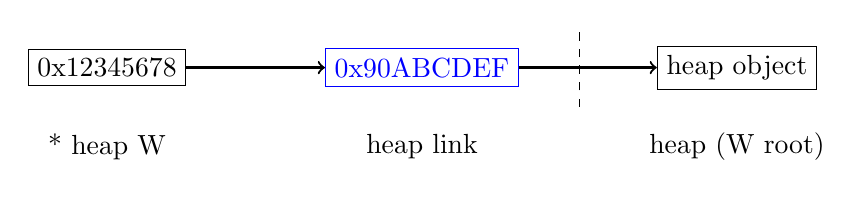
\begin{tikzpicture}
      \node [rectangle, draw] (p2) at (0,0) {0x12345678};
      \node at (0,-1) {* heap W};
      \node [rectangle, draw,blue] (hl) at (4,0) {0x90ABCDEF};
      \node at (4,-1) {heap link};
      \node [rectangle, draw] (heap) at (8,0) {heap object};
      \node at (8,-1) {heap (W root)};
      \draw [->,thick] (p2) -- (hl);
      \draw [->,thick] (hl) -- (heap);
      \draw [dashed] (6, -.5) -- (6, .5);
    \end{tikzpicture}

  \end{center}
\end{frame}

%% \begin{frame}

%%   Heaps may form hierarchies

%%   \vspace*{12pt}

%%   \begin{tikzpicture}
%%     [heap/.style={draw, rounded corners}]
%%     \node[heap] {component}
%%     child {
%%       node [heap] {heap1}
%%     }
%%     child {
%%       node [heap] {heap2}
%%       child {
%%         node [heap] {heap3}
%%       }
%%       child {
%%         node [heap] {heap4}
%%       }
%%     }
%%     ;
%%   \end{tikzpicture}

%% \end{frame}

\begin{frame}[fragile]{I/O}
  \begin{block}{Problem}
    Interact with external systems (through operating system)
  \end{block}

  \begin{block}{Challenges}
    \begin{itemize}
      \item Maintain fairness
      \item Avoid accidental sharing of state
    \end{itemize}
  \end{block}

  \begin{block}{Approach}
    \begin{enumerate}
    \item Introduce \verb+FileDescriptor+ type.
    \item Wrap \verb+FileDescriptor+s in reactive components.
    \item Introduce \verb+readable+ and \verb+writable+ predicates.
    \item Introduce functions for manipulating \verb+FileDescriptor+s.  All operations are non-blocking to ensure fairness.
    \end{enumerate}
  \end{block}
\end{frame}

\begin{frame}{Example:  Simple Network Time Protocol (SNTP)}
  \resizebox{\textwidth}{!}{
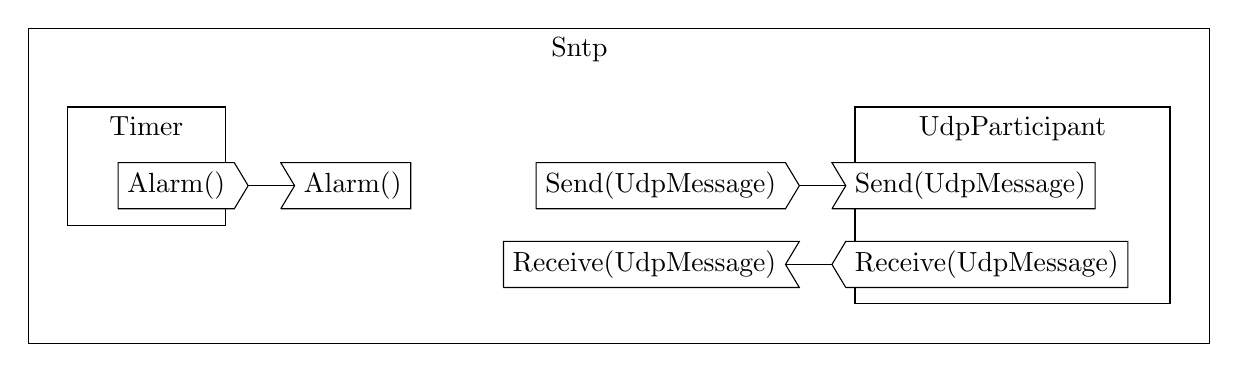
\begin{tikzpicture}
\draw (2,7.5) rectangle (4,9);
\node[below] at (3,9) {Timer};
\node (alarma) [shape=rightout, draw, fill=white] at (4,8) {Alarm()};

\draw (1.5,6) rectangle (16.5,10);
\node[below] at (8.5,10) {Sntp};
\node (alarmb) [shape=leftin, draw, fill=white] at (5,8) {Alarm()};
\node (senda)  [shape=rightout, draw, fill=white] at (11,8) {Send(UdpMessage)};
\node (receivea) [shape=rightin, draw, fill=white] at (11,7) {Receive(UdpMessage)};

\draw (12,6.5) rectangle (16,9);
\node[below] at (14,9) {UdpParticipant};
\node (sendb) [shape=leftin, draw, fill=white] at (12,8) {Send(UdpMessage)};
\node (receiveb) [shape=leftout, draw, fill=white] at (12,7) {Receive(UdpMessage)};

\draw (alarma.east) -- (alarmb.west);
\draw (senda.east) -- (sendb.west);
\draw (receiveb.west) -- (receivea.east);

\end{tikzpicture}
}
\end{frame}

\begin{frame}[fragile]{Example:  UdpParticipant}
\begin{lstlisting}
type UdpParticipant component {
  fd FileDescriptor;
  outQueue Queue;
  inQueue Queue;
  Receive push (msg $foreign UdpMessage);
}

init (this *UdpParticipant) Init () {
  this.fd = udp_socket()
}
\end{lstlisting}


\onslide<2>
\begin{tikzpicture}[overlay,remember picture]
  \pgftransformshift{\pgfpointanchor{current page}{center}}
  \node[
    rectangle callout,
    draw=eclipseGreen,
    ultra thick,
    fill=white,
    decorate,
    callout absolute pointer={(-1,1.8)},
    font=\Large,
    text width=0.6\textwidth,
    align=center,
    anchor=center
  ] at (2.5,0) {wrap a \verb+FileDescriptor+};
\end{tikzpicture}

\onslide<3>
\begin{tikzpicture}[overlay,remember picture]
  \pgftransformshift{\pgfpointanchor{current page}{center}}
  \node[
    rectangle callout,
    draw=eclipseGreen,
    ultra thick,
    fill=white,
    decorate,
    callout absolute pointer={(-.1,-1.1)},
    font=\Large,
    text width=0.6\textwidth,
    align=center,
    anchor=center
  ] at (2.5,0) {initialize a \verb+FileDescriptor+};
\end{tikzpicture}

\end{frame}

\begin{frame}[fragile]{Example:  UdpParticipant}
\begin{lstlisting}
reaction (this $const * UdpParticipant)
Send (msg $foreign UdpMessage) {
  var m UdpMessage = msg.Copy ();
  activate {
    this.outQueue.Push (m);
  };
}

action (this $const * UdpParticipant)
_send (!this.outQueue.Empty () &&
       writable (this.fd)) {
  activate {
    var m UdpMessage = this.outQueue.Front ();
    sendto (this.fd, m.host, m.port, m.msg);
    this.outQueue.Pop ();
  }
}
\end{lstlisting}

\onslide<2>
\begin{tikzpicture}[overlay,remember picture]
  \pgftransformshift{\pgfpointanchor{current page}{center}}
  \node[
    rectangle callout,
    draw=eclipseGreen,
    ultra thick,
    fill=white,
    decorate,
    callout absolute pointer={(.25,-.75)},
    font=\Large,
    text width=0.6\textwidth,
    align=center,
    anchor=center
  ] at (2.5,.75) {check status in precondition};
\end{tikzpicture}

\onslide<3>
\begin{tikzpicture}[overlay,remember picture]
  \pgftransformshift{\pgfpointanchor{current page}{center}}
  \node[
    rectangle callout,
    draw=eclipseGreen,
    ultra thick,
    fill=white,
    decorate,
    callout absolute pointer={(-3.1,-2)},
    font=\Large,
    text width=0.6\textwidth,
    align=center,
    anchor=center
  ] at (2.5,.75) {expose operating system calls};
\end{tikzpicture}

\end{frame}

%% \begin{frame}[fragile]{Example:  UdpParticipant}
%% \begin{lstlisting}
%% action (this $const * UdpParticipant)
%% _pre_receive (readable (this.fd)) {
%%   activate {
%%     var buf [64]byte;
%%     var r int = read(this.fd, buf[:]);
%%     var m UdpMessage;
%%     m.msg = copy(buf[0:r]);
%%     this.inQueue.Push (m);
%%   }
%% }

%% action (this $const *UdpParticipant)
%% _receive (!this.inQueue.Empty ()) {
%%   activate Receive (this.inQueue.Front ()) {
%%     this.inQueue.Pop ();
%%   }
%% }
%% \end{lstlisting}
%% \end{frame}

\begin{frame}{The Scheduling Problem}

  \begin{columns}
    \begin{column}{.5\textwidth}
      \resizebox{\textwidth}{!}{
      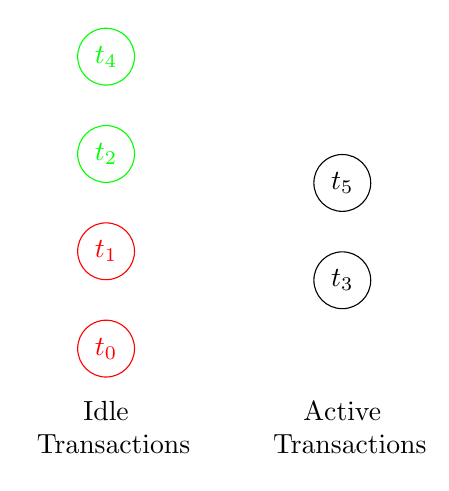
\begin{tikzpicture}
        [trans/.style={
            circle,
            draw,
            on chain},
          start chain=going above,
          node distance = .5cm]
        \node[text centered, text width=5em] at (0,0) {Idle \\ Transactions};
        \node[trans,red] at (0,1) {$t_0$};
        \node[trans,red] {$t_1$};
        \node[trans,green] {$t_2$};
        \node[trans,green] {$t_4$};

        \node[text centered, text width=5em] at (3,0) {Active \\ Transactions};
        \node[trans] at (3,1) {$t_3$};
        \node[trans] {$t_5$};
      \end{tikzpicture}
      }
    \end{column}
    \begin{column}{.5\textwidth}
      Pick an idle transaction that is {\color{green}safe} with respect to the set of active transactions subject to \emph{fairness}.
    \end{column}
  \end{columns}

\end{frame}

\begin{frame}{Scheduler Classes}

  When are preconditions evaluated?
  \begin{itemize}
  \item before execution (\emph{lazy}) or after execution (\emph{eager})
  \end{itemize}

  \vspace*{12pt}

  How is safety checked?
  \begin{itemize}
  \item every time (\emph{oblivious}) or never (\emph{knowledgeable})
  \end{itemize}

  \vspace*{12pt}

  How are race conditions handled?
  \begin{itemize}
  \item avoid (\emph{cautious}) or recover (\emph{speculative})
  \end{itemize}

  \vspace*{12pt}

  Is the execution of a transaction physically atomic?
  \begin{itemize}
  \item yes (\emph{non-preemptive}) or no (\emph{preemptive})
  \end{itemize}

\end{frame}

\begin{frame}{Scheduler Implementation}

  \begin{columns}
    \begin{column}[T]{.5\textwidth}

      \centering

      {\Large Instance Scheduler}

      \vspace*{8pt}

      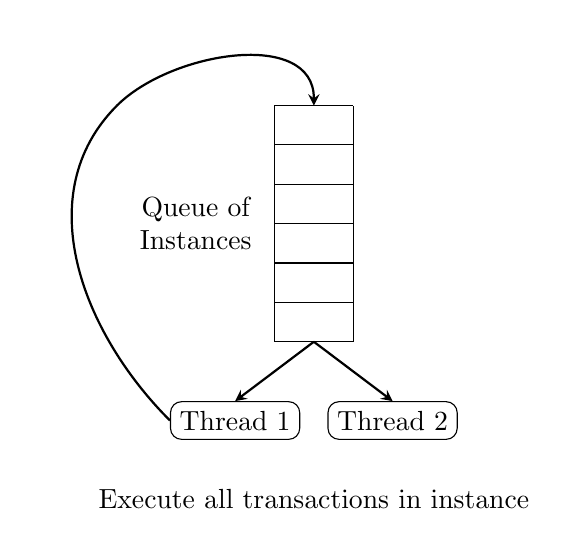
\begin{tikzpicture}
        [thread/.style={draw, rounded corners}]
        %\draw[help lines] (-2,-2) grid (2,4);
        \draw[ystep=.5cm] (0,0) grid (1,3);
        \node[text centered, text width=2cm] at (-1,1.5) {Queue of Instances};
        \node[thread] (t1) at (-.5,-1) {Thread 1};
        \node[thread] (t2) at (1.5,-1) {Thread 2};
        \draw[->,thick,>=stealth] (.5,0) -> (t1.north);
        \draw[->,thick,>=stealth] (.5,0) -> (t2.north);
        \node at (.5,-2) {Execute all transactions in instance};
        \draw[thick] (t1.west) to[out=135,in=225] (-2,3);
        \draw[->,thick,>=stealth] (-2,3) to[out=45,in=90] (.5,3);
      \end{tikzpicture}

    \end{column}
    \begin{column}[T]{.5\textwidth}

      \centering

      {\Large Partitioned Scheduler}

      \vspace*{8pt}

      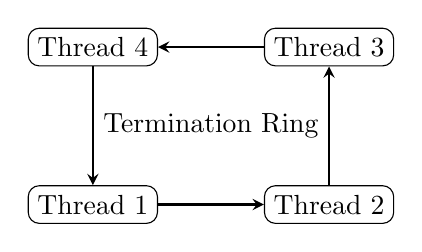
\begin{tikzpicture}
        [thread/.style={draw, rounded corners}]
        %\draw[help lines] (-2,-2) grid (2,4);
        \node[thread] (t1) at (0,0) {Thread 1};
        \node[thread] (t2) at (3,0) {Thread 2};
        \node[thread] (t3) at (3,2) {Thread 3};
        \node[thread] (t4) at (0,2) {Thread 4};
        \draw[->,thick,>=stealth] (t1.east) -- (t2.west);
        \draw[->,thick,>=stealth] (t2.north) -- (t3.south);
        \draw[->,thick,>=stealth] (t3.west) -- (t4.east);
        \draw[->,thick,>=stealth] (t4.south) -- (t1.north);
        \node at (1.5, 1) {Termination Ring};
      \end{tikzpicture}

      \vspace*{8pt}

      Thread

      \vspace*{8pt}

      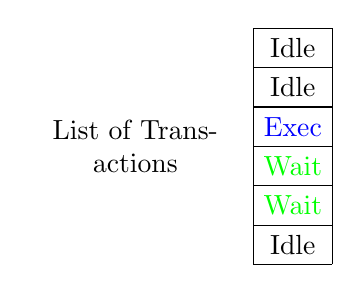
\begin{tikzpicture}
        \draw[ystep=.5cm] (0,0) grid (1,3);
        \node[text centered, text width=2.5cm] at (-1.5,1.5) {List of Transactions};
        \node at (.5, 2.75) {Idle};
        \node at (.5, 2.25) {Idle};
        \node[blue] at (.5, 1.75) {Exec};
        \node[green] at (.5, 1.25) {Wait};
        \node[green] at (.5,  .75) {Wait};
        \node at (.5,  .25) {Idle};
      \end{tikzpicture}

    \end{column}
  \end{columns}

\end{frame}

\begin{frame}{Scheduler Evaluation: AsyncClock \includegraphics[height=12pt]{CLOCK01-300px.png}}

  \begin{columns}
    \begin{column}{.4\textwidth}
      \begin{itemize}
      \item Machine:  2 cores
      \item Instance/Partitioned:  2 threads
      \item Thread:  3 threads
      \end{itemize}

      \vspace*{8pt}

      \emph{Thread suffers excessive context switches}
    \end{column}
    \begin{column}{.6\textwidth}
      \includegraphics[width=.6\textheight]{async_throughput_box.png}
    \end{column}
  \end{columns}

  \vspace*{12pt}

  \fbox{
    \parbox{\linewidth}{
      \centering
      Instance/Partitioned are viable event schedulers!
    }
  }

\end{frame}

\begin{frame}{Scheduler Evaluation: SyncClock \includegraphics[height=12pt]{CLOCK01-300px.png}}

    \begin{columns}
    \begin{column}{.4\textwidth}
      \begin{itemize}
      \item Machine:  2 cores
      \item Instance/Partitioned:  2 threads
      \item Thread:  \emph{2 threads}
      \end{itemize}
    \end{column}
    \begin{column}{.6\textwidth}
      \includegraphics[width=.6\textheight]{sync_throughput_box.png}
    \end{column}
  \end{columns}

  \vspace*{12pt}

  \fbox{
    \parbox{\linewidth}{
      \centering
      Compilation beats interpretation!
    }
  }

\end{frame}

\begin{frame}{Conclusions and Future Work}
  \begin{block}{Conclusions}
    \begin{enumerate}
    \item Reactive component model enables principled composition/decomposition of reactive systems.
    \item Reactive component semantics can be checked efficiently.
    \item Empirical results suggest that reactive components could compete with optimized multi-threaded approaches.
    \end{enumerate}
  \end{block}

  \begin{block}{Future Work}
    \begin{itemize}
    \item Extend model for introduction and dynamic composition
    \item Explore additional scheduler classes and algorithms
    \end{itemize}
  \end{block}
\end{frame}

\begin{frame}
  \centering
  \Huge
  Questions?
\end{frame}

%% \begin{frame}{\rcgo{}:  Reference Semantics}

%% \rcgo{} is a \emph{race-free} programming language

%% \resizebox{\textwidth}{!}{%
%% \begin{tikzpicture}
%% [
%%   >=stealth',
%%   punkt/.style={
%%     rectangle,
%%     rounded corners,
%%     draw=black, very thick,
%%     text width=6.5em,
%%     minimum height=2em,
%%     text centered
%%   },
%%   pil/.style={
%%     ->,
%%     thick,
%%     %%shorten <=2pt,
%%     %%shorten >=2pt,
%%   }
%% ]

%% %% stacks
%% \node[punkt] (stack1) at (0, 0) {Stack 1};
%% \node[punkt,below=4cm of stack1] (stack2) {Stack 2};
%% \node[below=1cm of stack2] (stackdots) {...};
%% \node[punkt,below=1cm of stackdots] (stacks) {Stack S};

%% %% components
%% \node[punkt,right=1cm of stack1] (component1) {Component 1};
%% \node[punkt,below=4cm of component1] (component2) {Component 2};
%% \node[below=1cm of component2] (componentdots) {...};
%% \node[punkt,below=1cm of componentdots] (componentc) {Component C};

%% %% heaps
%% \node[punkt, text width=4.5em,below=1cm of component1] (heap1) {Heap 1};
%% \node[punkt] (heap2) at ($(component1) + (6,3)$) {Transferable Heap 1};
%% \node[punkt, below=1cm of heap2] (heap3) {Transferable Heap 2};
%% \node[below=1cm of heap3] (heapdots) {...};
%% \node[punkt, below=1cm of heapdots] (heaph) {Transferable Heap H};

%% \node[punkt] (heap21) at ($(heaph) + (-2,-2)$) {Transferable Heap H.1};
%% \node[punkt] (heap22) at ($(heaph) + (2,-2)$) {Transferable Heap H.2};

%% \draw[pil,->] (stack1) -- (component1);
%% \draw[pil,->] (stack1) -- (component2.north west);
%% \draw[pil,->] (stack1) -- (heap1.north west);
%% \draw[pil,->] (stack1) -- (heap2.west);

%% \draw[pil,<->] (component1.south) -- (heap1.north);
%% \draw[pil,->] (component1.east) -- (heap2.west);
%% \draw[pil,->] (component1.east) -- (heap3.west);
%% \draw[pil,->] (heap1.east) -- (heaph.west);

%% \draw[pil,->] (heaph) -- (heap21.north);
%% \draw[pil,->] (heaph) -- (heap22.north);

%% \path[pil] (stack1.west) edge [loop above, out=-135, in=135, min distance=1.5cm] (stack1.west);
%% \path[pil] (stack2.west) edge [loop above, out=-135, in=135, min distance=1.5cm] (stack2.west);
%% \path[pil] (stacks.west) edge [loop above, out=-135, in=135, min distance=1.5cm] (stacks.west);

%% \path[pil] (component1.north) edge [loop above, out=135, in=45, min distance=1.5cm] (component1.north);
%% \path[pil] (component2.north) edge [loop above, out=135, in=45, min distance=1.5cm] (component2.north);
%% \path[pil] (componentc.north) edge [loop above, out=135, in=45, min distance=1.5cm] (componentc.north);

%% \path[pil] (heap1.south) edge [loop above, out=-45, in=-135, min distance=1.5cm] (heap1.south);
%% \path[pil] (heap2.east) edge [loop above, out=45, in=-45, min distance=1.5cm] (heap2.east);
%% \path[pil] (heap3.east) edge [loop above, out=45, in=-45, min distance=1.5cm] (heap3.east);
%% \path[pil] (heaph.east) edge [loop above, out=45, in=-45, min distance=1.5cm] (heaph.east);

%% \path[pil] (heap21.east) edge [loop above, out=45, in=-45, min distance=1.5cm] (heap21.east);
%% \path[pil] (heap22.east) edge [loop above, out=45, in=-45, min distance=1.5cm] (heap22.east);

%% \end{tikzpicture}
%% }

%% \end{frame}

%% \makeatletter
%% \pgfdeclareshape{clock}
%% {%
%%   % All anchors are taken from the 'circle' shape:
%%   \inheritsavedanchors[from={circle}]%
%%   \inheritanchor[from={circle}]{center}%
%%   \inheritanchor[from={circle}]{mid}%
%%   \inheritanchor[from={circle}]{base}%
%%   \inheritanchor[from={circle}]{north}%
%%   \inheritanchor[from={circle}]{south}%
%%   \inheritanchor[from={circle}]{west}%
%%   \inheritanchor[from={circle}]{east}%
%%   \inheritanchor[from={circle}]{mid west}%
%%   \inheritanchor[from={circle}]{mid east}%
%%   \inheritanchor[from={circle}]{base west}%
%%   \inheritanchor[from={circle}]{base east}%
%%   \inheritanchor[from={circle}]{north west}%
%%   \inheritanchor[from={circle}]{south west}%
%%   \inheritanchor[from={circle}]{north east}%
%%   \inheritanchor[from={circle}]{south east}%
%%   \inheritanchorborder[from={circle}]%
%%   %
%%   % Only the background path is different
%%   %
%%   \backgroundpath{%
%%     % First the existing 'circle' code:
%%     \pgfutil@tempdima=\radius%
%%     \pgfmathsetlength{\pgf@xb}{\pgfkeysvalueof{/pgf/outer xsep}}%
%%     \pgfmathsetlength{\pgf@yb}{\pgfkeysvalueof{/pgf/outer ysep}}%
%%     %% \ifdim\pgf@xb<\pgf@yb%
%%     %%   \advance\@tempdima by-\pgf@yb%
%%     %% \else%
%%     %%   \advance\@tempdima by-\pgf@xb%
%%     %% \fi%
%%     \pgfpathcircle{\centerpoint}{\@tempdima}%
%%     %
%%     % Now the | and -- lines:
%%     \pgfmoveto{\centerpoint}%
%%     \pgflineto{\pgfpointscale{.5}{\pgfpointadd{\centerpoint}{\pgfpoint{0pt}{\pgfutil@tempdima}}}}%
%%     \pgfmoveto{\centerpoint}%
%%     \pgflineto{\pgfpointscale{.5}{\pgfpointadd{\centerpoint}{\pgfpoint{\pgfutil@tempdima}{0pt}}}}%
%%   }%
%% }
%% \makeatother

%% \begin{frame}

%%   trends slide - IIOT

%%   DDS to introduce problems with state of the art

%%   Contributions

%%   model

%%   \begin{center}
%%     {\LARGE Synchronous Reactive Systems}
%%     \vspace*{12pt}

%%     \begin{tikzpicture}
%%       \node at (0,2) {0};
%%       \node at (1,2) {1};
%%       \node at (2,2) {2};
%%       \node at (3,2) {3};
%%       \node at (4,2) {4};
%%       \node at (5,2) {5};
%%       \node at (6,2) {6};

%%       \fill[red] (1,1.25) rectangle (3,1.75);
%%       \fill[red] (4,1.25) rectangle (5,1.75);
%%       \draw (0,1.25) rectangle (6,1.75);

%%       \fill[blue] (0,.25) rectangle (4,.75);
%%       \fill[blue] (5,.25) rectangle (6,.75);
%%       \draw (0,.25) rectangle (6,.75);

%%       \draw[fill] (-1.5,1) circle [radius=.5];
%%       \draw[white] (-1.5,1) -- (-1.5,1.5);
%%       \draw[white] (-1.5,1) -- (-1, 1);
%%       \draw (-1,1) -- (-.5,1);
%%       \draw (-.5,1) -- (-.5,1.5);
%%       \draw (-.5,1) -- (-.5,.5);
%%       \draw (-.5,1.5) -- (0, 1.5);
%%       \draw (-.5,.5) -- (0, .5);
%%     \end{tikzpicture}
%%   \end{center}

%%   \rule{\textwidth}{0.4pt}

%%   \begin{center}
%%     {\LARGE Asynchronous Reactive Programs}
%%     \vspace*{12pt}

%%     \begin{tikzpicture}
%%       \draw[fill] (-1,1.5) circle [radius=.25];
%%       \draw[white] (-1,1.5) -- (-1,1.75);
%%       \draw[white] (-1,1.5) -- (-.75, 1.5);

%%       \draw[fill] (-1,.5) circle [radius=.25];
%%       \draw[white] (-1,.5) -- (-1,.75);
%%       \draw[white] (-1,.5) -- (-.75, .5);

%%       \draw (-.75,1.5) -- (6, 1.5);
%%       \draw (-.75,.5) -- (6, .5);


%%       \draw[fill,red] (0,1.5) circle [radius=.1];
%%       \draw[fill,red] (1,1.5) circle [radius=.1];
%%       \draw[fill,red] (2,1.5) circle [radius=.1] node (a) {};
%%       %\draw[fill,red] (3,1.5) circle [radius=.1];
%%       \draw[fill,red] (4,1.5) circle [radius=.1];
%%       \draw[fill,red] (5,1.5) circle [radius=.1];
%%       \draw[fill,red] (6,1.5) circle [radius=.1];

%%       \draw[fill,blue] (0,.5) circle [radius=.1];
%%       \draw[fill,blue] (.5,.5) circle [radius=.1];
%%       \draw[fill,blue] (1,.5) circle [radius=.1];
%%       \draw[fill,blue] (2.5,.5) circle [radius=.1] node (b) {};
%%       \draw[fill,blue] (3.5,.5) circle [radius=.1];
%%       \draw[fill,blue] (4,.5) circle [radius=.1];
%%       \draw[fill,blue] (6,.5) circle [radius=.1];

%%       \draw[->,>=stealth'] (a) -- (b) {};

%%       \node[draw, shape=ellipse, minimum height=2cm, minimum width=1cm] (so) at (2.25,1) {};

%%       \node () at (2.25, -.5) {synchronization};
%%     \end{tikzpicture}
%%   \end{center}
%% \end{frame}

%% \begin{frame}
%%   \frametitle{Limitations of the State of the Art}

%%   show a picture of a DDS like application

%%   show deadlock

%%   highlight the burden placed on programmer
%%   \begin{enumerate}
%%   \item identify and protect shared state
%%   \item understand the call graph
%%   \end{enumerate}

%% \end{frame}

\end{document}
